%======================================================================
%  Technical background notes: LLM inference on HBM-equipped CPUs
%  Build from the repository root with:
%      inv notes
%======================================================================
\documentclass[11pt,a4paper]{article}

\usepackage[margin=2.6cm]{geometry}
\usepackage[T1]{fontenc}
\usepackage{lmodern}
\usepackage{microtype}
\usepackage{amsmath}
\usepackage{amssymb}
\usepackage{graphicx}
\graphicspath{{figures/}}
\usepackage{booktabs}
\usepackage{tabularx}
\usepackage{xltabular}
\usepackage{array}
\usepackage{xcolor}
\usepackage{enumitem}
\usepackage{caption}
\usepackage{float}
\usepackage{flafter}
\usepackage{placeins}
\usepackage{tikz}
\usetikzlibrary{arrows.meta, positioning, fit, calc}
\usepackage{listings}
\usepackage{xurl}
\usepackage[numbers,sort&compress]{natbib}
\usepackage{colortbl}
\usepackage[colorlinks=true, linkcolor=seccol, urlcolor=accent,
            citecolor=citecol]{hyperref}

\definecolor{accent}{RGB}{128,0,32}
\definecolor{hbmcol}{RGB}{213,125,28}
\definecolor{ddrcol}{RGB}{55,105,165}
\definecolor{neutralcol}{RGB}{235,238,242}

%  One colour per class of cross-reference, so a reader can tell at a
%  glance whether a link points to a source, a figure, a table or an
%  equation.
\definecolor{citecol}{RGB}{128,0,32}   % sources
\definecolor{figcol}{RGB}{27,102,74}   % figures
\definecolor{tabcol}{RGB}{35,82,145}   % tables
\definecolor{eqcol}{RGB}{112,54,132}   % equations
\definecolor{seccol}{RGB}{85,85,95}    % sections
\definecolor{tabhead}{RGB}{236,239,244}
\definecolor{tabband}{RGB}{248,249,251}

\newcolumntype{Y}{>{\raggedright\arraybackslash}X}
\newcolumntype{P}[1]{>{\raggedright\arraybackslash}p{#1}}
\setlist[itemize]{leftmargin=*, itemsep=2pt, topsep=4pt}
\setlist[enumerate]{leftmargin=*, itemsep=2pt, topsep=4pt}
\captionsetup{font=small, labelfont=bf}
\captionsetup[figure]{labelfont={bf,color=figcol}}
\captionsetup[table]{labelfont={bf,color=tabcol}}
\setlength{\emergencystretch}{2em}
\widowpenalty=10000
\clubpenalty=10000

%  Float placement.  The defaults are far too willing to push a float
%  onto a page of its own and stretch the surrounding text to fill the
%  gap; these let floats sit where they are written.
\raggedbottom
\setcounter{topnumber}{3}
\setcounter{bottomnumber}{2}
\setcounter{totalnumber}{4}
\renewcommand{\topfraction}{0.9}
\renewcommand{\bottomfraction}{0.7}
\renewcommand{\textfraction}{0.07}
\renewcommand{\floatpagefraction}{0.75}
\setlength{\textfloatsep}{14pt plus 3pt minus 3pt}
\setlength{\intextsep}{13pt plus 3pt minus 3pt}

%  Cross-reference commands.  Each prints its own kind in its own
%  colour; \ref* keeps the link from nesting.
\newcommand{\figref}[1]{\hyperref[#1]{\textcolor{figcol}{Figure~\ref*{#1}}}}
\newcommand{\tabref}[1]{\hyperref[#1]{\textcolor{tabcol}{Table~\ref*{#1}}}}
\newcommand{\eqnref}[1]{\hyperref[#1]{\textcolor{eqcol}{Equation~\ref*{#1}}}}
\newcommand{\secref}[1]{\hyperref[#1]{\textcolor{seccol}{Section~\ref*{#1}}}}

%  A caption for a displayed equation, styled like a figure caption so
%  that equations can be referred to by name in the text.
\newcommand{\eqcaption}[1]{%
  \par\vspace{-2pt}%
  \begingroup
    \small
    \setlength{\baselineskip}{12.5pt}%
    \noindent\textcolor{eqcol}{\textbf{Equation~\theequation:}}~#1\par
  \endgroup
  \vspace{9pt}}

%  Table furniture: a tinted header row and a little more breathing
%  room between rows.
\newcommand{\headrow}{\rowcolor{tabhead}}
\newcommand{\tabsetup}{\renewcommand{\arraystretch}{1.22}}

\lstdefinestyle{shell}{
  language=bash,
  basicstyle=\ttfamily\footnotesize,
  backgroundcolor=\color{neutralcol},
  frame=single,
  rulecolor=\color{black!25},
  framerule=0.4pt,
  columns=fullflexible,
  keepspaces=true,
  breaklines=true,
  showstringspaces=false,
  aboveskip=8pt,
  belowskip=8pt
}

\newcommand{\lcpp}{\texttt{llama.cpp}}
\newcommand{\ggml}{\texttt{ggml}}

\title{\textbf{Technical Background and Experimental Rationale}\\[5pt]
       \Large LLM Inference on HBM-Equipped CPUs\\[3pt]
       \large The CRESCO8 Xeon Max Platform}
\author{}
\date{}

\begin{document}
\maketitle

%  Bibliography ordering.  natbib's plainnat sorts alphabetically and
%  mixes research literature with vendor documentation; unsrtnat instead
%  follows the order in which entries are first cited, and the \nocite
%  block below is read before any prose, so it fixes that order.  Research
%  literature comes first, then the technical and institutional sources
%  that are cited for facts rather than for findings.
\nocite{agrawal2025evaluating, arif2026inferencescaling, bi2026rooflinebench,
        chen2025ktransformers, chen2026memorybound, dongarra2026gpus,
        fang2025kvplacement, goto2026aurorahpl, he2024distributedcpu,
        ibeid2025aurora, jang2026hymcache, jang2026itme,
        kurt2026quantization, li2024hardwareperspective,
        lu2026thinfer, malakhov2025medlocalgpt, na2024llmcpu,
        peng2017hybridmemory, reguly2023xeonmax, salaria2025metametrics,
        shen2023efficientcpu, stuhlmann2025bench360,
        wei2025tmac, williams2009roofline, yuan2024roofline,
        zhang2024nomad, zhang2026cacheresident, zuo2026fairyfuse}
\nocite{cresco8doc, eneacresco8slides, eneapress, intel9480, intelmax,
        intelmaxtuning, llamacpp2026, lp1603}

\begin{abstract}
\noindent
Quantized language-model inference on CPUs has become ordinary practice,
and the work that made it so has been overwhelmingly arithmetic:
fewer bits per weight, cheaper kernels, better use of the matrix units.
That line of attack is now visibly saturating: a recent ternary kernel
reports a thirty-fold improvement in isolation and a 1.24-fold
improvement end to end, which suggests the binding constraint has
moved to data movement.  The Intel Xeon CPU Max~9480 is
an unusually direct place to test that suggestion, because it exposes
on-package HBM2e and DDR5 as separately addressable memory tiers on one
socket, so placement becomes a page policy rather than a data transfer.

These notes assemble the background for a thesis built on that
observation, using the fifteen HBM-equipped nodes of the CRESCO8 cluster
at ENEA Portici.  They describe the Xeon Max memory hierarchy and the
testbed, develop a step-level performance model for prefill and
autoregressive decode, and review the two literatures the question sits
between: CPU inference, which has concentrated on arithmetic, and
memory tiering, which has strong measured results in HPC but has reached
transformer inference mainly through simulation or through
accelerator-attached hierarchies.  The central experimental comparison
is local HBM against local DDR5 on the same socket in Flat mode, with
prefill and sustained decode reported separately; comparisons across
processors are secondary because they move several variables at once.
Working-set capacity, arithmetic intensity, memory-level parallelism and
verified page residency are treated throughout as the quantities that
decide whether a bandwidth advantage becomes a performance advantage.
The final part turns this into a reproducible experimental design.
\end{abstract}

\tableofcontents

\clearpage
\part{Experimental platform}
%======================================================================
%  What a cluster is, and which part of one this thesis uses
%======================================================================

\section{Supercomputers, clusters and nodes}
\label{sec:hpc-primer}

\subsection{What makes a machine a supercomputer}

A modern supercomputer is not a single very large computer.  It is a
few hundred to a few thousand ordinary computers, wired together and
managed as one facility.  Each of those computers, called a \textbf{node}, has its own
processors, its own memory and its own operating system, and looks from
the inside much like a well-specified server.  What turns
a room full of nodes into a supercomputer is the three things bolted
around them: a fast \textbf{interconnect} so that nodes can exchange
data, a \textbf{parallel file system} they all see, and a
\textbf{scheduler} that hands nodes out to users a job at a time.

\figref{fig:workstation-vs-cluster} contrasts this with the machine on
a desk.  The important difference is not size but \emph{addressability}.
On a workstation, every core can read every byte of memory directly.  On
a cluster that remains true \emph{within} a node and stops being true
between nodes: to use another node's memory, a program has to send a
message over the network and wait.  Crossing that boundary is roughly
three orders of magnitude more expensive than a local memory access, and
almost everything difficult about parallel programming follows from it.

\begin{figure}[htbp]
\centering
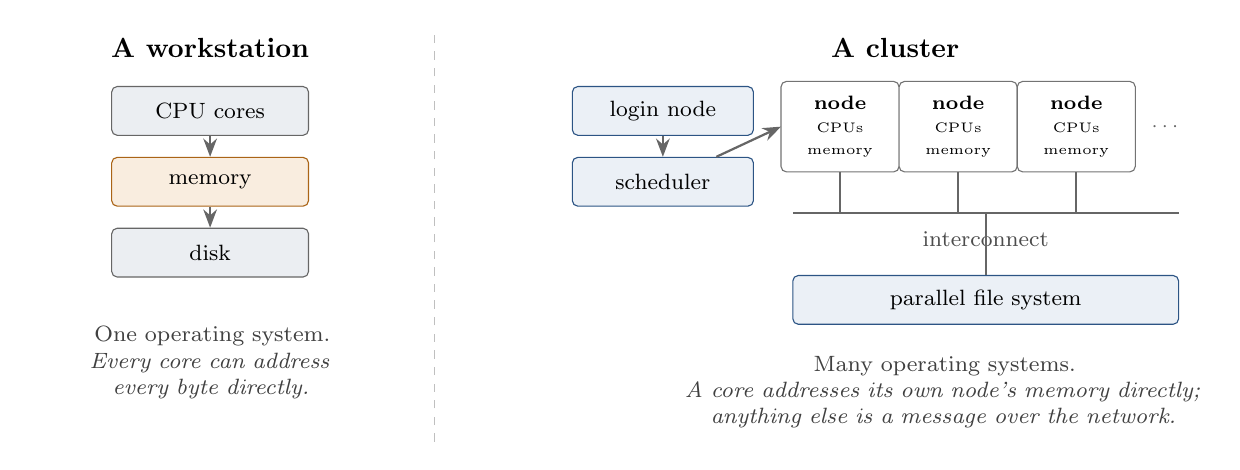
\begin{tikzpicture}[
  font=\small,
  box/.style={draw=black!60, fill=neutralcol, rounded corners=2pt,
              minimum width=2.5cm, minimum height=0.62cm, align=center,
              font=\footnotesize},
  nodebox/.style={draw=black!55, fill=white, rounded corners=2pt,
                  minimum width=1.5cm, minimum height=1.15cm,
                  align=center, font=\scriptsize},
  svc/.style={draw=ddrcol!80!black, fill=ddrcol!10, rounded corners=2pt,
              minimum width=2.3cm, minimum height=0.62cm, align=center,
              font=\footnotesize},
  lbl/.style={font=\footnotesize, align=center},
  lnk/.style={-{Stealth}, thick, black!60}
]
  % workstation side
  \node[font=\bfseries] at (-4.4,3.05) {A workstation};
  \node[box] (wc) at (-4.4,2.25) {CPU cores};
  \node[box, fill=hbmcol!14, draw=hbmcol!80!black] (wm) at (-4.4,1.35)
    {memory};
  \node[box] (wd) at (-4.4,0.45) {disk};
  \draw[lnk] (wc) -- (wm);
  \draw[lnk] (wm) -- (wd);
  \node[lbl, text width=4.4cm, black!75] at (-4.4,-0.95)
    {One operating system.\\\emph{Every core can address\\every byte
     directly.}};

  \draw[black!25, dashed] (-1.55,-1.95) -- (-1.55,3.3);

  % cluster side
  \node[font=\bfseries] at (4.3,3.05) {A cluster};
  \node[svc] (login) at (1.35,2.25) {login node};
  \node[svc] (sched) at (1.35,1.35) {scheduler};
  \draw[lnk] (login) -- (sched);

  \foreach \i/\x in {1/3.6, 2/5.1, 3/6.6} {
    \node[nodebox] (n\i) at (\x,2.05)
      {\textbf{node}\\{\tiny CPUs}\\{\tiny memory}};
  }
  \node[font=\scriptsize, black!60] at (7.75,2.05) {$\cdots$};

  \draw[lnk] (sched) -- (2.85,2.05);
  \draw[black!60, thick] (3.0,0.95) -- (7.9,0.95);
  \foreach \x in {3.6,5.1,6.6} \draw[black!60, thick] (\x,1.47) -- (\x,0.95);
  \node[lbl, black!70] at (5.45,0.62) {interconnect};

  \node[svc, minimum width=4.9cm] (fs) at (5.45,-0.15)
    {parallel file system};
  \draw[black!60, thick] (5.45,0.95) -- (5.45,0.16);

  \node[lbl, text width=6.6cm, black!75] at (4.9,-1.32)
    {Many operating systems.\\\emph{A core addresses its own node's
     memory directly;\\anything else is a message over the network.}};
\end{tikzpicture}
\caption{A workstation and a cluster, drawn to show where direct memory
addressing stops.  The dashed line is the boundary this thesis works
inside: all of the experiments run on \emph{one} node, so the
interconnect and the scheduler are context rather than subject.
Author's synthesis.}
\label{fig:workstation-vs-cluster}
\end{figure}

\subsection{How a cluster is used}

Access follows a fixed shape, and it is worth stating because it
constrains the experimental method described in Part~III.  A user logs
in to a \textbf{login node}, which is shared, modest, and meant for
editing and compiling rather than for running anything.  Work is then
submitted to a \textbf{batch scheduler}, which on CRESCO8 is Slurm, as
a script that declares what it needs: how many nodes, how
many cores, for how long, from which partition.  The scheduler queues
the request, and when the resources free up it runs the script on the
allocated nodes and returns the output.

Two consequences matter here.  First, \emph{measurements are taken
without an interactive session}, so anything the experiment needs to
record must be written down by the job script at the time; there is no
opportunity to inspect the machine afterwards.  Second, \emph{the
allocation is not the whole machine}.  A job receives specific nodes
from a specific partition, and the properties of those nodes, rather than
the properties advertised for the cluster, are what a result depends
on.  This is why \secref{sec:first-allocation} treats capturing a
machine-readable system manifest as the first task of the first
allocation rather than as housekeeping.

\subsection{Why HPC hardware differs from a desktop}

Nodes in a cluster are built for sustained throughput rather than for
peak responsiveness, and the differences show up in exactly the places
this thesis cares about.  They carry two or more processor sockets, so
memory access time depends on which socket a thread runs on.  They
carry many more memory channels than a desktop, because feeding fifty
or a hundred cores takes considerably more bandwidth than feeding
eight.  They are cooled aggressively, on CRESCO8 with water, so that high core
counts can be sustained rather than briefly reached.  And
increasingly they carry \emph{more than one kind of memory}, which is
where this thesis begins.

That last point is the reason a cluster appears in a study of language
model inference at all.  The processor examined here, the Intel Xeon CPU
Max~9480, is a mainstream server CPU with an unusual property: it has
high-bandwidth memory in the package alongside ordinary DDR5, and both
can be addressed by software.  Machines built from it are rare, and
essentially all of them are supercomputers.  Studying the question
therefore requires cluster access even though the question itself is
about a single socket.

\subsection{What this thesis actually uses}

The funnel narrows quickly, and \tabref{tab:hpc-scope} states where it
stops.  Of everything above, the experiments use one node from one
partition, and the primary comparison uses one socket of that node.  The
interconnect is never on the critical path.  The parallel file system
matters only for storing model files.  The scheduler matters only
because it decides which node is obtained and for how long.

\begin{table}[htbp]
\centering
\small
\tabsetup
\caption{Which parts of the cluster this thesis depends on.  The
narrowness is deliberate: every level that is excluded is a level whose
variability cannot contaminate the memory-tier comparison.}
\label{tab:hpc-scope}
\begin{tabularx}{\textwidth}{@{}P{3.05cm}P{3.3cm}Y@{}}
\toprule
\headrow
\textbf{Level} & \textbf{Role in this thesis} & \textbf{Why} \\
\midrule
Cluster
& \textbf{Context only}
& Provides access to a processor that is otherwise unobtainable, and
  imposes the queue limits that shape the experiment matrix. \\
\addlinespace[1pt]
Interconnect
& \textbf{Excluded}
& All experiments are single-node, so network performance never enters
  a reported measurement. \\
\addlinespace[1pt]
File system
& \textbf{Support only}
& Holds model files; excluded from every timing boundary. \\
\addlinespace[1pt]
Scheduler
& \textbf{Method}
& Determines which node is allocated, which is why the observed node
  configuration, not the documented one, is what gets reported. \\
\addlinespace[1pt]
Node
& \textbf{Secondary subject}
& Two sockets joined by UPI; used for the topology questions, where
  crossing between sockets is the effect being measured. \\
\addlinespace[1pt]
\textbf{Socket}
& \textbf{Primary subject}
& \emph{The unit on which the central comparison is defined.}  One set
  of cores, one local HBM tier, one local DDR5 tier. \\
\bottomrule
\end{tabularx}
\end{table}

With that scope fixed, the next two sections work inwards:
\secref{sec:xeon-max-platform} describes the socket and the memory
system that make the question askable, and \secref{sec:cresco8}
describes the particular cluster on which it will be asked.

%======================================================================
%  Hardware platform: SD650 V3 and Intel Xeon CPU Max
%======================================================================

\section{Xeon Max and the SD650 V3}
\label{sec:xeon-max-platform}

\subsection{The unit of analysis}

The Lenovo ThinkSystem SD650~V3 is a dense, direct-water-cooled server
tray rather than a single compute node.  One tray contains two
independent dual-socket nodes, and six trays fit in a 6U DW612S
enclosure~\cite{lp1603}.  This distinction matters when reporting
quantities: the CRESCO8 allocation is a \emph{node}; memory locality is
defined first at the \emph{socket}; and the scheduler may allocate
individual cores within the node.  \tabref{tab:hardware-hierarchy} sets
out the four levels and what each one is good for.

\begin{table}[htbp]
\centering
\small
\tabsetup
\caption{Hardware hierarchy and the properties relevant to this study.
Product capability is separated from the installed CRESCO8
configuration described in \secref{sec:cresco8}
~\cite{lp1603,cresco8doc}.}
\label{tab:hardware-hierarchy}
\begin{tabularx}{\textwidth}{@{}lYY@{}}
\toprule
\headrow
\textbf{Level} & \textbf{Composition} & \textbf{Relevance} \\
\midrule
DW612S enclosure
  & Six SD650~V3 trays (12 independent nodes)
  & Shared power and cooling infrastructure; not an allocation unit. \\
SD650~V3 tray
  & Two independent dual-socket nodes
  & High-density packaging; the two nodes do not form one shared-memory
    system. \\
Compute node
  & Two Xeon processors connected by Intel UPI
  & Scheduler allocation and the largest cache-coherent NUMA system used
    by the single-node experiments. \\
Xeon Max socket
  & CPU cores, 64\,GB on-package HBM2e and eight DDR5 channels
  & Primary locality domain and the cleanest unit for comparing HBM with
    DDR5. \\
\bottomrule
\end{tabularx}
\end{table}

The product guide covers several processor, memory, storage and network
options.  Most of those options are irrelevant to the thesis.  The
important configuration is the Xeon CPU Max 9480 installed on CRESCO8:
56 physical cores per socket, 64\,GB of HBM2e, eight DDR5-4800 channels,
and four UPI links~\cite{intel9480,lp1603}.  A two-socket node therefore
provides 112 physical cores and 128\,GB of nominal HBM capacity.  The
node also contains DDR5, but its installed capacity and channel
population are properties of CRESCO8, not of the product family.

\begin{figure}[htbp]
\centering
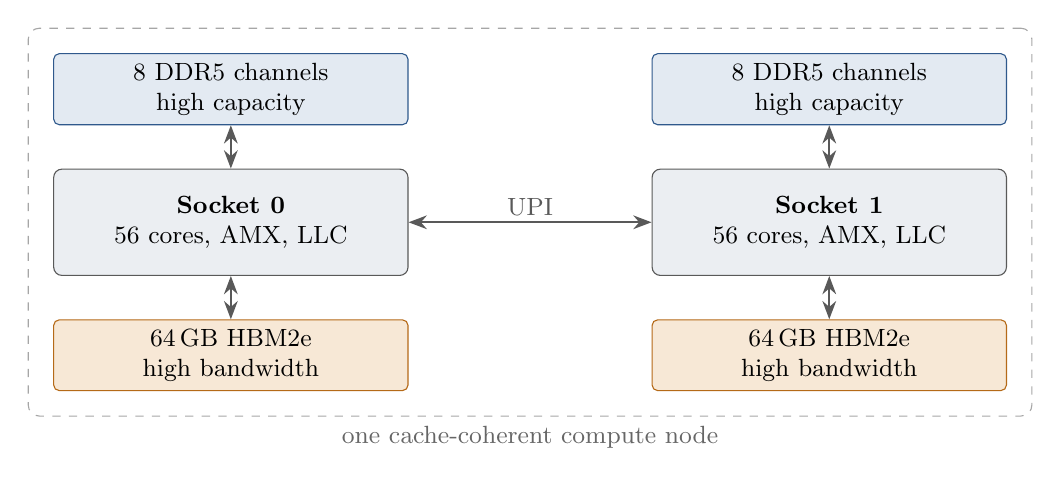
\begin{tikzpicture}[
  font=\small,
  socket/.style={draw=black!65, fill=neutralcol, rounded corners=3pt,
                 minimum width=4.5cm, minimum height=1.35cm,
                 align=center},
  hbm/.style={draw=hbmcol!85!black, fill=hbmcol!18, rounded corners=2pt,
              minimum width=4.5cm, minimum height=0.85cm, align=center},
  ddr/.style={draw=ddrcol!85!black, fill=ddrcol!14, rounded corners=2pt,
              minimum width=4.5cm, minimum height=0.85cm, align=center},
  link/.style={{Stealth}-{Stealth}, thick, black!65}
]
  \node[socket] (s0) at (-3.8,0)
    {\textbf{Socket 0}\\56 cores, AMX, LLC};
  \node[socket] (s1) at (3.8,0)
    {\textbf{Socket 1}\\56 cores, AMX, LLC};
  \node[hbm, below=0.55cm of s0] (h0)
    {64\,GB HBM2e\\high bandwidth};
  \node[hbm, below=0.55cm of s1] (h1)
    {64\,GB HBM2e\\high bandwidth};
  \node[ddr, above=0.55cm of s0] (d0)
    {8 DDR5 channels\\high capacity};
  \node[ddr, above=0.55cm of s1] (d1)
    {8 DDR5 channels\\high capacity};

  \draw[link] (s0) -- node[above, fill=white, inner sep=2pt]{UPI} (s1);
  \draw[link] (s0) -- (h0);
  \draw[link] (s1) -- (h1);
  \draw[link] (s0) -- (d0);
  \draw[link] (s1) -- (d1);

  \node[draw=black!35, dashed, rounded corners=4pt, inner sep=9pt,
        fit=(d0)(d1)(h0)(h1),
        label={[black!60]below:{one cache-coherent compute node}}] {};
\end{tikzpicture}
\caption{Conceptual locality map of a CRESCO8 Xeon Max node.  Each
socket has local HBM and DDR5; access to the other socket traverses UPI.
The diagram represents locality, not physical package routing.
Author's synthesis based on the platform and cluster documentation
~\cite{lp1603,cresco8doc}.}
\label{fig:node-locality}
\end{figure}


\subsection{What the hardware looks like}
\label{sec:hardware-photographs}

Three photographs from the product documentation make
\tabref{tab:hardware-hierarchy} concrete.  They are worth a moment,
because the packaging explains several constraints that reappear later
as experimental limitations.

\begin{figure}[htbp]
\centering
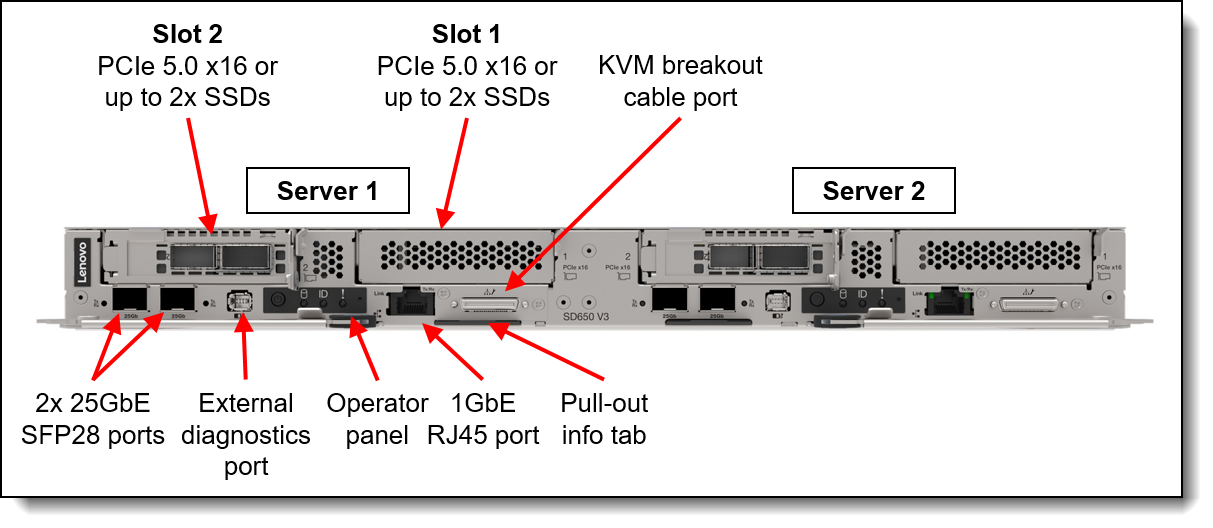
\includegraphics[width=0.94\textwidth]{sd650v3-front-view.png}
\caption{Front of one SD650~V3 tray.  The two servers are independent
computers that happen to share a chassis: each has its own network
ports, its own operator panel and its own management interface, and
they share only power and water.  What is \emph{not} present is as
informative as what is.  There is no video output, no removable media
and no local console, because a node of this kind is never approached
directly.  Reproduced from the Lenovo ThinkSystem SD650~V3 product
guide~\cite{lp1603}.}
\label{fig:sd650-front}
\end{figure}

\figref{fig:sd650-front} shows the tray from the front.  Two servers,
side by side, each with a pair of 25\,GbE ports for the high-speed
fabric and a 1\,GbE port for management.  The experiments in this thesis
touch none of these interfaces: work arrives through the scheduler and
results leave through the file system.

\begin{figure}[htbp]
\centering
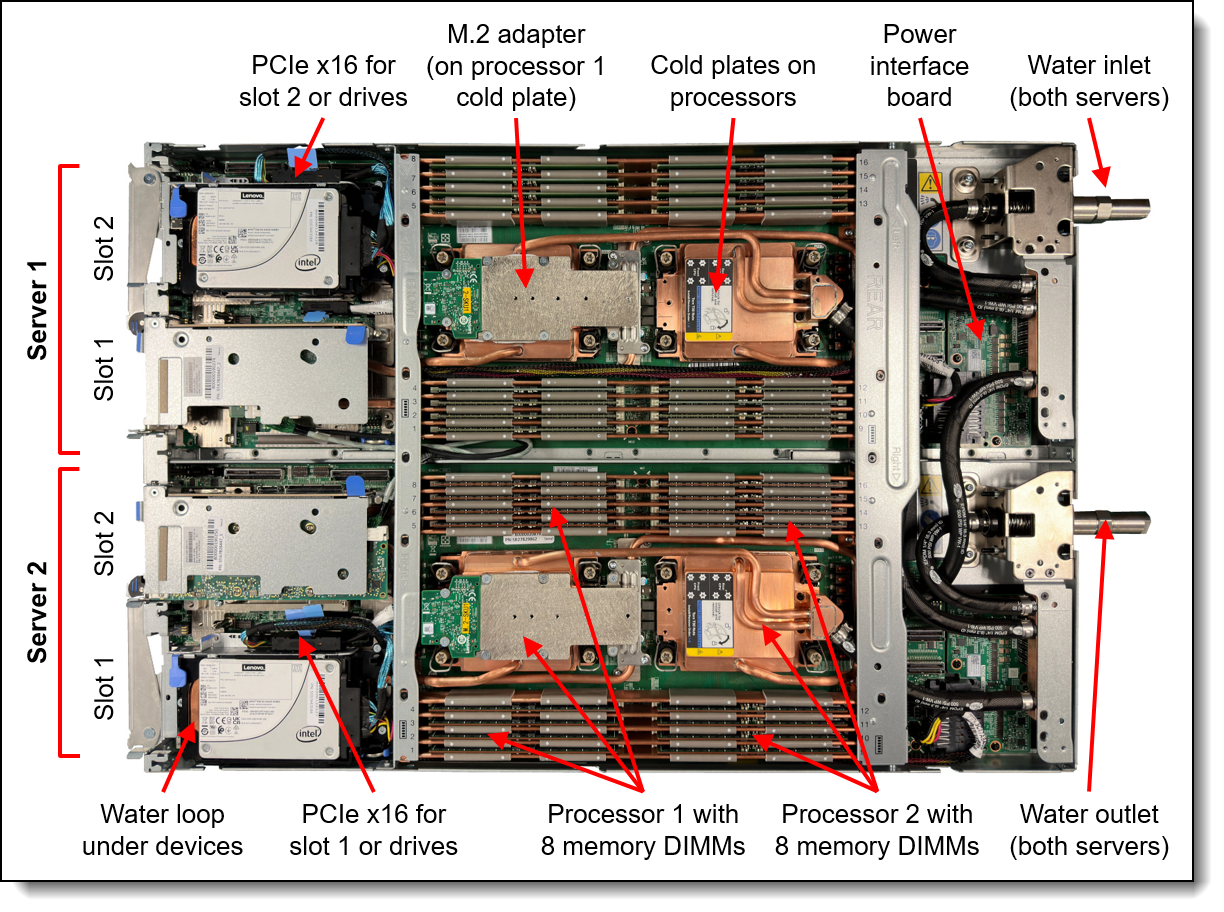
\includegraphics[width=0.94\textwidth]{sd650v3-internal-view.png}
\caption{Inside the tray.  Each of the two servers carries two
processors, and each processor is flanked by eight memory DIMMs.  The
copper cold plates and the loop that joins them replace the fans
entirely.  The high-bandwidth memory that this thesis is about is
nowhere visible: it sits inside the processor package, beneath the cold
plate, which is why its capacity is fixed and why it cannot be
configured, replaced or upgraded.  Reproduced from the Lenovo
ThinkSystem SD650~V3 product guide~\cite{lp1603}.}
\label{fig:sd650-internal}
\end{figure}

\figref{fig:sd650-internal} is the more useful of the two.  The layout
of one server, two processors with their own DIMMs on either side, is
the physical form of the locality argument made throughout this section:
a thread running on the left-hand processor reaches the DIMMs beside it
quickly and the DIMMs on the right slowly, and no amount of software can
change the distance.  The absence of fans is also visible, and it
matters for measurement rather than for acoustics, since a water-cooled
socket holds its clock under sustained load instead of ramping fans and
throttling.

\begin{figure}[htbp]
\centering
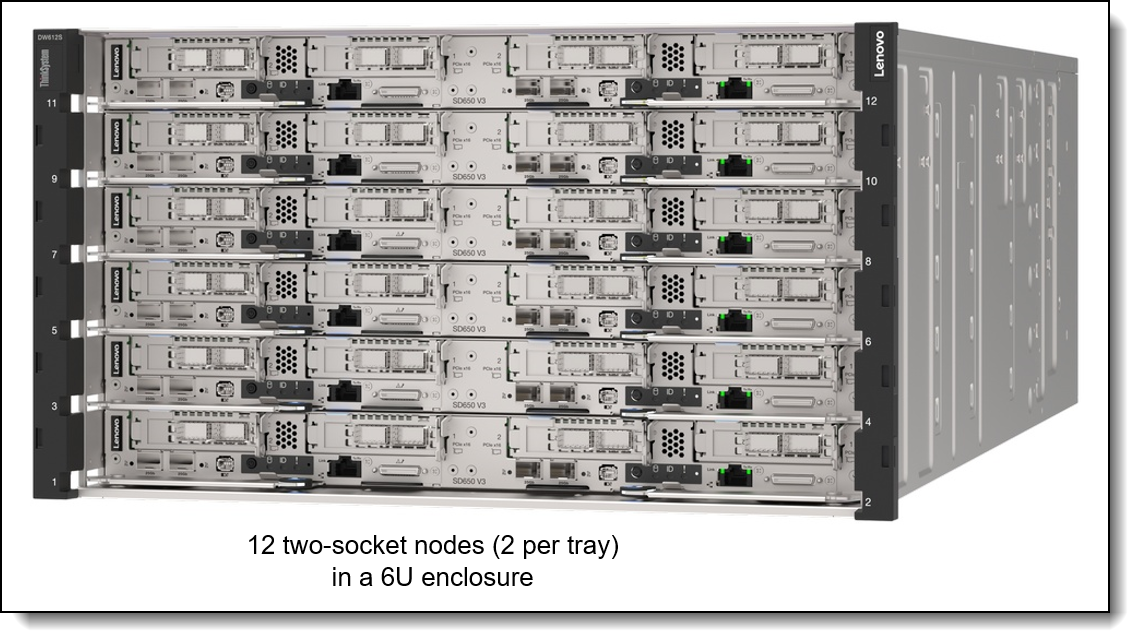
\includegraphics[width=0.80\textwidth]{dw612s-enclosure-nodes.png}
\caption{Six trays in one 6U DW612S enclosure, giving twelve independent
two-socket nodes.  A scheduler allocation yields one of these, not the
enclosure and not the rack.  Reproduced from the Lenovo ThinkSystem
SD650~V3 product guide~\cite{lp1603}.}
\label{fig:dw612s-enclosure}
\end{figure}

\figref{fig:dw612s-enclosure} completes the picture: twelve nodes in one
enclosure, and a few dozen enclosures in the machine room.  A job that
asks for a node receives one of the trays in this photograph, with its
neighbours in the enclosure running unrelated work.  That is the reason
\secref{sec:first-allocation} insists on recording which node was
obtained.

\subsection{Compute capability, and why it is not the binding constraint}

Xeon Max is a Sapphire Rapids processor with conventional x86 cores,
AVX-512, and Intel Advanced Matrix Extensions (AMX).  AMX adds per-core
tile registers and matrix-multiply instructions for BF16 and INT8
operands~\cite{intelmax,na2024llmcpu}, and on well-shaped
matrix--matrix products it is a large win, which is why prompt
processing benefits from it and single-token generation largely does
not.

The detail that matters for a quantized workload is what AMX does not
provide.  There is no native INT4 dot-product instruction, so a 4-bit
GGUF model cannot be fed to the matrix engine in the format it is stored
in.  \figref{fig:amx-path} shows the consequence: every weight must
pass through an unpack and dequantize step before it reaches a tile, and
that step sits precisely between the memory tier and the matrix unit.
The arrangement has an awkward property for this thesis.  Lower-bit
formats reduce the bytes moved, which is what makes them attractive on a
bandwidth-limited machine, but they add work on the path from memory to
the matrix engine, and they push the operand format further from
anything the engine can consume directly.  Whether a given model
benefits from AMX at all therefore depends on the runtime, the storage
format, the packing scheme and the matrix dimensions, none of which are
properties of the processor.

\begin{figure}[htbp]
\centering
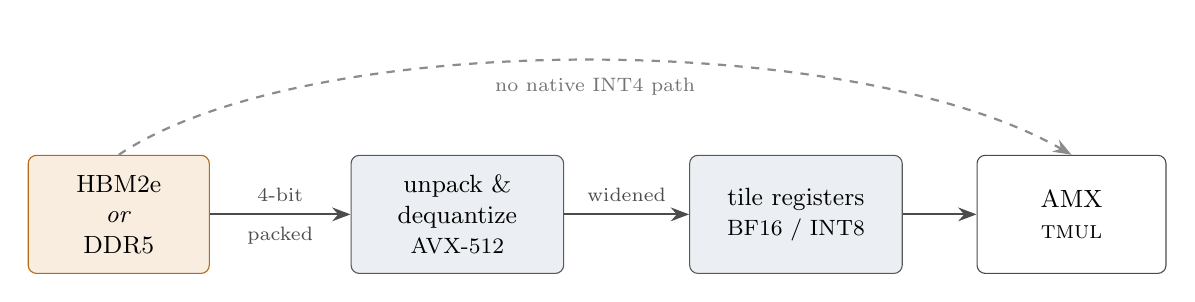
\begin{tikzpicture}[
  font=\small,
  mem/.style={draw=hbmcol!85!black, fill=hbmcol!14, rounded corners=3pt,
              minimum width=2.3cm, minimum height=1.5cm, align=center},
  stage/.style={draw=black!65, fill=neutralcol, rounded corners=3pt,
                minimum width=2.7cm, minimum height=1.5cm, align=center},
  eng/.style={draw=black!70, fill=white, rounded corners=3pt,
              minimum width=2.4cm, minimum height=1.5cm, align=center},
  flow/.style={-{Stealth}, thick, black!70},
  edgelbl/.style={font=\scriptsize, align=center, text=black!70}
]
  \node[mem]   (m) at (0,0)    {HBM2e\\\emph{or}\\DDR5};
  \node[stage] (u) at (4.3,0)  {unpack \&\\dequantize\\{\footnotesize AVX-512}};
  \node[stage] (t) at (8.6,0)  {tile registers\\{\footnotesize BF16 / INT8}};
  \node[eng]   (x) at (12.1,0) {AMX\\\textsc{tmul}};

  \draw[flow] (m) -- node[above=1pt, edgelbl] {4-bit}
                    node[below=1pt, edgelbl] {packed} (u);
  \draw[flow] (u) -- node[above=1pt, edgelbl] {widened} (t);
  \draw[flow] (t) -- (x);

  \draw[dashed, thick, black!45, -{Stealth}]
    (m.north) .. controls +(2.4,1.6) and +(-2.8,1.6) .. (x.north);
  \node[edgelbl, text=black!55, fill=white, inner sep=2pt] at (6.05,1.62)
    {no native INT4 path};
\end{tikzpicture}
\caption{Path taken by a quantized weight from a memory tier to the
matrix engine on Xeon Max.  The unpack stage is unavoidable for 4-bit
formats and lies between the two things this thesis compares.  At batch
one the right-hand operand is a vector, so the tile is largely empty and
the engine runs far below its rated throughput; the step is paced
instead by the arrival of weights from the left.  Author's synthesis
from the Xeon Max product documentation and the AMX description in Na et
al.~\cite{intelmax,na2024llmcpu}.}
\label{fig:amx-path}
\end{figure}

\textbf{Peak instruction throughput is not an application result.}  Small
matrices, batch-one matrix--vector operations, packing overhead and
memory stalls can all leave the matrix units idle, and the advertised
maximum turbo frequency is a single-core limit rather than the frequency
of a socket running sustained AMX kernels.  Frequency, package power and
throttling state have to be observed during the experiments rather than
read off a specification table.


\subsection{The memory hierarchy}
\label{sec:memory-hierarchy}

HBM and DDR5 trade different resources.  HBM provides much greater
aggregate bandwidth and 64\,GB of nominal capacity per socket.  DDR5
provides substantially more capacity and can have lower unloaded access
latency.  HBM is therefore not simply ``faster memory''.  It is most valuable
under two conditions that have to hold \emph{together}: the workload
issues enough concurrent requests to approach its bandwidth, \emph{and}
the bandwidth-critical working set is placed locally.  Either one alone
is not enough.

Published STREAM results illustrate both the advantage and the need for
local measurement.  Na et al.\ report 588\,GB/s for HBM and
233.8\,GB/s for DDR5 on a Xeon Max 9468 socket
~\cite{na2024llmcpu}.  Ibeid et al.\ report 680--840\,GB/s for HBM and
235--245\,GB/s for DDR5 on a related Xeon Max 9470C
~\cite{ibeid2025aurora}.  These sustained values are 2.5--3.4 times
apart, but the HBM results themselves differ by more than 15\%.  SKU,
clustering mode, thread placement and benchmark configuration are
plausible causes.  None of these numbers should be used as the bandwidth
of CRESCO8 before the Max 9480 nodes are measured.

Three paths must be distinguished in every result:

\begin{itemize}
  \item \textbf{local HBM or local DDR5}, reached from cores on the same
        socket;
  \item \textbf{remote memory}, reached through UPI from the other
        socket; and
  \item \textbf{mixed placement}, in which pages, threads or model
        objects span several locality domains.
\end{itemize}

\figref{fig:node-locality} draws these three paths.  An apparently
node-wide 128\,GB HBM allocation is consequently two 64\,GB local
tiers.  A workload uses the aggregate capacity and
bandwidth only if data and computation are balanced across sockets.

\begin{table}[htbp]
\centering
\small
\tabsetup
\caption{Storage levels visible to one Max 9480 socket, ordered by the
question that matters here: who decides what occupies them.  Only the
last three rows are under software control, and only in Flat mode.
Cache capacities follow the SKU specification and should be confirmed
with \texttt{lscpu} on the allocated node~\cite{intel9480,lp1603}.}
\label{tab:storage-levels}
\begin{tabularx}{\textwidth}{@{}P{2.35cm}P{3.05cm}P{3.15cm}Y@{}}
\toprule
\headrow
\textbf{Level} & \textbf{Capacity} & \textbf{Placement decided by} &
\textbf{Why it matters here} \\
\midrule
L1 data & 48\,KB per core & Hardware & Too small to hold any part of a
  weight tensor. \\
L2 & 2\,MB per core & Hardware & Holds tiles and activations; invisible
  to a placement policy. \\
Last-level cache & 112.5\,MB, shared & Hardware replacement policy &
  The tier Zhang et al.\ target by rebuilding the
  runtime~\cite{zhang2026cacheresident}; not addressable directly. \\
\addlinespace[2pt]
HBM2e & 64\,GB, four stacks & \textbf{Software}, in Flat mode &
  The bandwidth tier, and the object of this study. \\
DDR5 & Eight channels; installed capacity is a CRESCO8 property &
  \textbf{Software}, in Flat mode & The capacity tier and the control
  condition. \\
Remote memory & The other socket's tiers & \textbf{Software}, through
  thread and page binding & Reached over UPI; a placement failure rather
  than a design choice. \\
\bottomrule
\end{tabularx}
\end{table}

\tabref{tab:storage-levels} also locates this thesis against the
closest competing work.
Zhang et al.\ obtain large gains by keeping weights resident in the
last-level cache~\cite{zhang2026cacheresident}, one row above the tier
studied here, but that row is not addressable, so their result required
rebuilding the runtime around it.  The HBM row can be
addressed directly, which is what makes the comparison in this thesis
possible without touching the runtime at all.

\subsection{Bandwidth is only reachable with enough concurrency}
\label{sec:littles-law}

A bandwidth number describes what the memory system can deliver when it
is kept busy, and nothing about whether a given program manages to keep
it busy.  The relationship is Little's law: the number of bytes a
program must have in flight to sustain a bandwidth \(B\) against a
latency \(L\) is

\begin{equation}
\label{eq:little}
  C = B \times L .
\end{equation}
\eqcaption{Little's law applied to a memory system.  It converts a bandwidth figure into a requirement on the program: this many bytes must be outstanding at every instant, or the bandwidth is unreachable no matter which tier holds the data.}

Substituting the published Xeon Max figures into \eqnref{eq:little}
makes the difference between the two tiers concrete.  For HBM at 840\,GB/s and 134.9\,ns, roughly
113\,KB must be outstanding at all times, which is about 1{,}770 cache
lines, or close to 32 lines per core across 56 cores.  For DDR5 at 245\,GB/s
and 112.9\,ns the requirement is roughly 28\,KB, about 430 lines, or
under 8 per core~\cite{ibeid2025aurora}.  The faster tier does not merely
offer \emph{more} bandwidth; it demands roughly \textbf{four times the
memory-level parallelism} before that bandwidth becomes reachable at
all.

That demand is not obviously satisfiable.  Thirty-two concurrent line
fills per core is the same order of magnitude as the outstanding-miss
resources a single core has available, so approaching HBM peak requires
almost every one of them to stay occupied, helped by hardware
prefetchers that work well on strided streams and poorly on dependent
ones.  The exact resource counts for this microarchitecture must be
confirmed rather than assumed, but the shape of the constraint does not
depend on the precise number.

This is the mechanism behind the most important negative result in the
tiered-memory literature.  Peng et al.\ found that HPC codes with
regular access patterns gained up to 3$\times$ from MCDRAM while codes
with irregular, latency-bound patterns could run \emph{slower} in the
high-bandwidth tier, and that adding hardware threads, which is to say adding concurrency,
recovered much of the loss~\cite{peng2017hybridmemory}.  Low-batch autoregressive decode has
exactly the awkward shape: the weight stream is regular and prefetchable,
but the dependent chain through each layer limits how far ahead the core
can run, and the attention path over a growing KV cache is less regular
still.

Two consequences follow for the experiments.  Thread count is not a
nuisance parameter to be fixed at ``all cores'' but a first-class
factor, because it directly sets available concurrency; and a
disappointing HBM result must be diagnosed by measuring achieved
bandwidth rather than reported as an absence of effect.  A run that
reaches 250\,GB/s on HBM has \emph{not} shown that HBM does not help;
it has shown that \textbf{the program never asked HBM for anything DDR5
could not also have delivered}.

\subsection{HBM memory modes}
\label{sec:hbm-modes}

Xeon Max supports three ways to expose HBM, shown side by side in
\figref{fig:hbm-modes}~\cite{lp1603,intelmaxtuning}.  The mode is
selected in firmware and is normally fixed for the lifetime of a boot.

\begin{figure}[htbp]
\centering
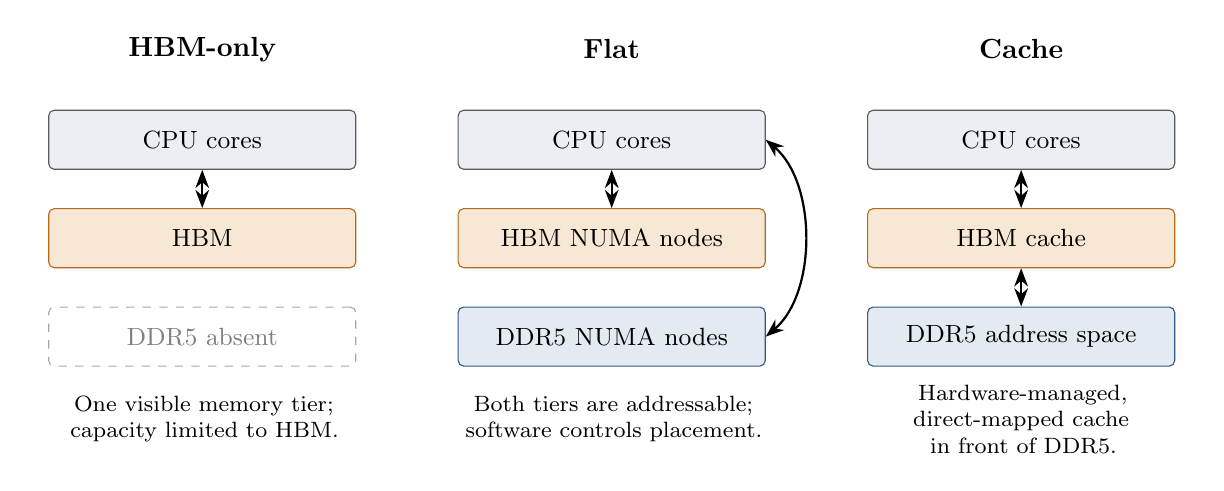
\begin{tikzpicture}[
  font=\small,
  cpu/.style={draw=black!65, fill=neutralcol, rounded corners=2pt,
              minimum width=3.9cm, minimum height=0.75cm, align=center},
  hbm/.style={draw=hbmcol!85!black, fill=hbmcol!18, rounded corners=2pt,
              minimum width=3.9cm, minimum height=0.75cm, align=center},
  ddr/.style={draw=ddrcol!85!black, fill=ddrcol!14, rounded corners=2pt,
              minimum width=3.9cm, minimum height=0.75cm, align=center},
  absent/.style={draw=black!35, dashed, text=black!50, rounded corners=2pt,
                 minimum width=3.9cm, minimum height=0.75cm, align=center},
  link/.style={{Stealth}-{Stealth}, thick},
  note/.style={font=\footnotesize, text width=4.2cm, align=center}
]
  \node[font=\bfseries] at (0,1.15) {HBM-only};
  \node[cpu] (c0) at (0,0) {CPU cores};
  \node[hbm] (h0) at (0,-1.25) {HBM};
  \node[absent] (d0) at (0,-2.5) {DDR5 absent};
  \draw[link] (c0) -- (h0);
  \node[note] at (0,-3.55)
    {One visible memory tier; capacity limited to HBM.};

  \node[font=\bfseries] at (5.2,1.15) {Flat};
  \node[cpu] (c1) at (5.2,0) {CPU cores};
  \node[hbm] (h1) at (5.2,-1.25) {HBM NUMA nodes};
  \node[ddr] (d1) at (5.2,-2.5) {DDR5 NUMA nodes};
  \draw[link] (c1) -- (h1);
  \draw[link] (c1.east) .. controls +(0.65,-0.55) and
                                  +(0.65,0.55) .. (d1.east);
  \node[note] at (5.2,-3.55)
    {Both tiers are addressable; software controls placement.};

  \node[font=\bfseries] at (10.4,1.15) {Cache};
  \node[cpu] (c2) at (10.4,0) {CPU cores};
  \node[hbm] (h2) at (10.4,-1.25) {HBM cache};
  \node[ddr] (d2) at (10.4,-2.5) {DDR5 address space};
  \draw[link] (c2) -- (h2);
  \draw[link] (h2) -- (d2);
  \node[note] at (10.4,-3.55)
    {Hardware-managed, direct-mapped cache in front of DDR5.};
\end{tikzpicture}
\caption{The three Xeon Max memory modes, shown for one socket.  Flat
mode is the only mode that exposes HBM and DDR5 as separately
controllable memory tiers.  Author's synthesis from the Xeon Max product
and tuning guides~\cite{lp1603,intelmaxtuning}.}
\label{fig:hbm-modes}
\end{figure}

\begin{description}
  \item[HBM-only mode.] The system contains no DDR5 and exposes HBM as
  ordinary system memory.  It is simple for software but imposes a hard
  capacity limit.  It is not the documented CRESCO8 configuration.

  \item[Flat mode.] HBM and DDR5 share the physical address space but
  appear as distinct NUMA memory nodes.  Applications can allocate
  directly from a tier, or an external policy can bind pages with
  \texttt{mbind}, libnuma or \texttt{numactl}.  Allocation is not enough:
  first touch, page migration and memory mapping can change actual page
  residency, which must be verified.

  \item[Cache mode.] HBM is a hardware-managed, direct-mapped cache in
  front of DDR5.  Applications see the DDR5 capacity without placing
  objects explicitly, but software cannot choose which objects remain
  in HBM.  Conflict misses, warm state and a working set near the cache
  capacity can make performance workload-dependent
  ~\cite{ibeid2025aurora}.
\end{description}

Flat mode provides the strongest experimental design because local HBM
and local DDR5 can be compared on the same socket without changing the
processor or executable.  A Flat-versus-Cache comparison answers a
different question: it measures explicit placement against a hardware
cache policy.

\subsection{Clustering and NUMA}

Memory mode is independent of the processor's clustering mode.  In
Quadrant mode, one socket is normally presented as one compute locality
domain.  Sub-NUMA Clustering (SNC4) exposes four domains per socket,
each associated with a subset of cores, cache, DDR channels and HBM.
SNC4 can increase bandwidth and reduce local latency for software that
places workers and data per quadrant, but it also makes remote accesses
easier to create.  In Flat+SNC4, the nominal 64\,GB HBM socket is divided
into four 16\,GB locality domains.

This distinction explains why a mode cannot be labelled universally
``best''.  Ibeid et al.\ obtain the highest STREAM bandwidth with SNC4
and explicit locality, whereas Na et al.\ observe worse inference
performance and more remote traffic under SNC4
~\cite{ibeid2025aurora,na2024llmcpu}.  The result depends on the
software's placement policy, not only on the processor setting.

\subsection{Cooling and instrumentation}

Direct water cooling allows two high-power processors to operate in a
dense node, but it does not guarantee a fixed frequency or energy
efficiency.  The relevant quantities are measured socket frequency,
temperature, package power and throttling state.  Product-guide claims
about facility heat recovery or cooling savings are not evidence about
inference performance.

\begin{figure}[htbp]
\centering
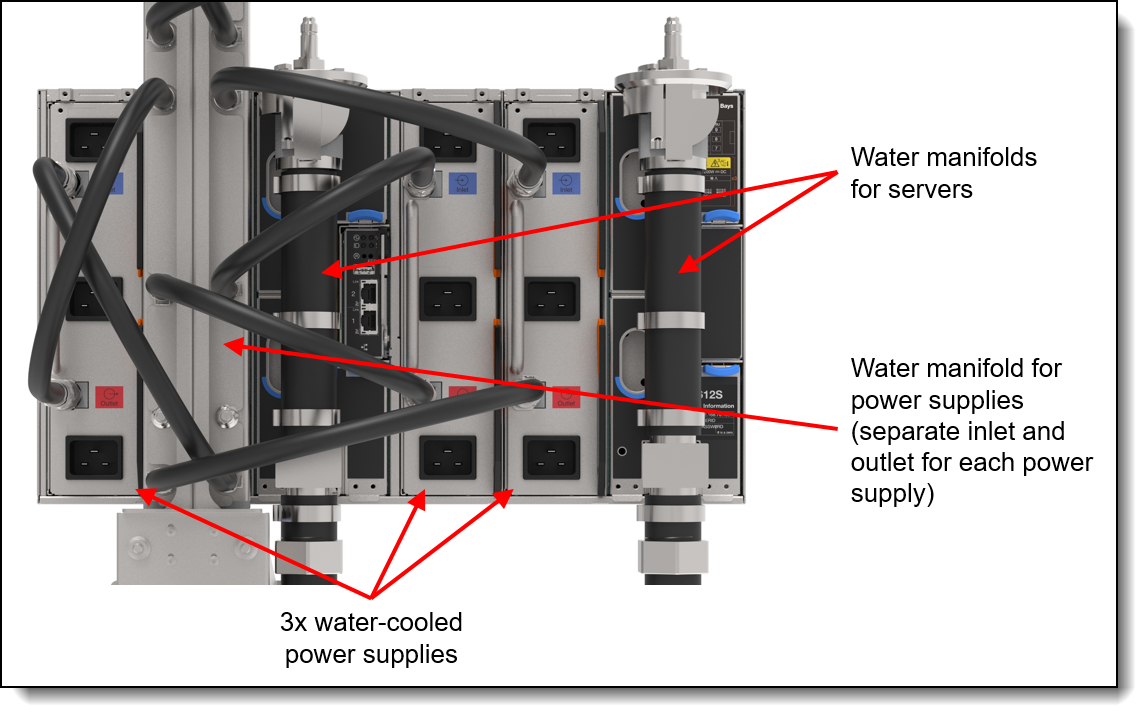
\includegraphics[width=0.82\textwidth]{dw612s-water-manifold.png}
\caption{Rear of the enclosure.  Water is distributed to the trays
through manifolds, and even the power supplies are water-cooled, so the
enclosure has no air path at all.  For this thesis the consequence is
narrow but useful: thermal conditions are set by facility water
temperature rather than by neighbouring workloads, which removes one
source of run-to-run variation.  Reproduced from the Lenovo ThinkSystem
SD650~V3 product guide~\cite{lp1603}.}
\label{fig:dw612s-manifold}
\end{figure}

\figref{fig:dw612s-manifold} shows how the water reaches the trays.
The SD650~V3 includes XClarity management and a TI INA226-based
power/energy meter with 100\,Hz sampling capability
~\cite{lp1603}.  This establishes a platform capability, not user
access on CRESCO8.  Intel RAPL, management-controller telemetry and
whole-node power meters cover different system boundaries; they must
not be combined without first validating their scope, units, sampling
and permissions.

\subsection{Consequences for the thesis}

Five requirements follow from the hardware, and each of them exists
because a specific thing can go wrong.

\begin{enumerate}
  \item Establish the active memory and clustering modes from the
        allocated node rather than from the product guide.  Flat mode is
        a precondition for the primary comparison, not a default.
  \item Measure sustained local HBM and DDR5 behaviour before drawing a
        Roofline or interpreting any inference result.  The published
        figures for this processor family differ by more than 15\%
        between studies, which is too much to inherit.
  \item Treat thread count as a factor rather than a constant.  It sets
        the memory-level parallelism available to the run, and therefore
        how much of the HBM bandwidth the workload can reach at all
        (\secref{sec:littles-law}).
  \item Bind threads and pages, then verify residency and remote traffic
        rather than trusting the command line.  A memory policy records
        an intention; only a page count records an outcome.
  \item Record frequency, thermal and power state throughout, so that a
        placement effect cannot be confused with a change in operating
        conditions.
\end{enumerate}

The common thread is that this processor offers several ways to obtain a
result that looks like a memory-tier effect and is not one.  Most of the
methodological weight in Part~III goes on ruling those out.

%======================================================================
%  CRESCO8 as the experimental testbed
%======================================================================

\section{CRESCO8 as the experimental testbed}
\label{sec:cresco8}

\subsection{Documented configuration}

CRESCO8 is the current CRESCO system at the ENEA research centre in
Portici.  It entered service in 2025 and is connected by a 200\,Gb/s
Mellanox NDR fabric~\cite{cresco8doc,eneapress}.  The operational user
page distinguishes the three compute-node classes listed in
\tabref{tab:cresco8-node-classes}:

\begin{table}[htbp]
\centering
\small
\tabsetup
\caption{CRESCO8 node classes documented by ENEAGRID.  Counts describe a
dated operational document, not a permanent scheduler inventory
~\cite{cresco8doc}.}
\label{tab:cresco8-node-classes}
\begin{tabularx}{\textwidth}{@{}lcccY@{}}
\toprule
\headrow
\textbf{Class} & \textbf{Nodes} & \textbf{CPU cores/node}
 & \textbf{Memory/node} & \textbf{Processor or accelerator} \\
\midrule
CPU
 & 760 & 128 & 512\,GB DDR5
 & 2$\times$ Xeon Platinum 8592+ \\
CPU--HBM
 & 15 & 112 & 1,024\,GB DDR5 + 128\,GB HBM
 & 2$\times$ Xeon CPU Max 9480 \\
GPU
 & 17 & 128 & 512\,GB DDR5 + accelerator HBM
 & 2$\times$ Xeon Platinum 8592+ and
   4$\times$ Intel Data Center GPU Max 1550 \\
\bottomrule
\end{tabularx}
\end{table}

The same page calls this a 793-node system, although the listed classes
sum to 792 and its reported core total is consistent with the 792-node
breakdown.  Earlier commissioning material gives yet another snapshot
~\cite{eneacresco8slides}.  This inconsistency is operational rather than scientific, and the
response is procedural: every experiment retains dated
\texttt{sinfo -N} and \texttt{scontrol show node} output, and the thesis
\textbf{reports the observed inventory} rather than silently reconciling
historical documents.


\subsection{Why the HBM partition supports a clean comparison}

Each documented HBM node contains two Max 9480 sockets, 1\,TB of DDR5
and 128\,GB of HBM.  This makes three comparisons possible, but they do
not have equal evidential strength:

\begin{enumerate}
  \item \textbf{Local HBM versus local DDR5 on the same Max 9480
        socket} is the primary comparison.  Processor, core count,
        executable and most firmware conditions can be held constant.

  \item \textbf{One socket versus two sockets, or Quadrant versus SNC4},
        tests the runtime's response to topology.  It is a placement
        experiment, not a pure memory-technology comparison.

  \item \textbf{Max 9480 versus Platinum 8592+} is a secondary
        system-level baseline.  The processors differ in generation,
        core count, cache, clocks, memory channels and uncore behaviour.
        The contrast cannot identify an HBM effect by itself.
\end{enumerate}

The installed DDR capacity does not reveal the DIMM layout.  Sixteen
64\,GB DIMMs would populate all channels, but the platform also permits
eight 128\,GB DIMMs with Xeon Max~\cite{lp1603}.  Channel population,
memory frequency and local bandwidth therefore require direct
inspection.  The presence of DDR5 also means that the nodes use Flat or
Cache mode rather than the no-DDR HBM-only configuration, but the ENEA
page does not identify which mode is active.  In Flat mode, HBM appears
as memory-only NUMA nodes; in Cache mode it does not appear separately.

The NDR link has a raw one-direction rate of 25\,GB/s per node, far
below local HBM bandwidth.  Multi-node inference may still be necessary
for capacity, but communication can then dominate the placement effect.
Single-node experiments should establish a stable result before adding
distributed parallelism.

\subsection{Scheduler and storage context}

The documented production partition is \texttt{cresco8\_hbm}, with 14
nodes and a 24-hour limit; \texttt{cresco8\_hbm\_dbg} lists two nodes
and a one-hour limit~\cite{cresco8doc}.  Their hostnames can overlap, so
these counts must not be added.

Compute nodes are reached only through Slurm.  The front ends are for
editing, compilation and submission, not benchmarking.  ENEAGRID
provides AFS for shared home directories and Lustre for parallel I/O;
large model files and benchmark output belong on the latter, subject to
the site's current mount points and quotas.  Compiler, MPI and profiler
modules listed on the web page are useful starting points, but an
experiment must record the modules and linked libraries actually loaded
on the run date.

\subsection{Why this platform, and what it costs}
\label{sec:why-cresco8}

Machines that expose HBM and DDR as separately addressable tiers on a
general-purpose CPU are not common, and the ones that exist are mostly
not reachable.  Aurora is the largest Xeon Max deployment and the source
of most of the published measurement literature on this
processor~\cite{ibeid2025aurora,goto2026aurorahpl}, but access to it is
not something a thesis can assume.  Fifteen nodes at ENEA are a small
resource by comparison, and for the question in
\secref{sec:research-gap} that hardly matters: the primary
comparison is defined on a single socket, and a single socket is what
the argument needs.  The scarce commodity here is \emph{not nodes but the processor
itself}.

The scarcity does shape the experimental design, though, and it is
better to admit that in the method than to discover it halfway through.
Fourteen nodes in \texttt{cresco8\_hbm} are shared with the rest of the
centre, the queue limit is 24 hours, and the debug partition offers two
nodes for an hour.  A full Cartesian sweep over model, quantization,
prompt length, generation length, batch size, thread count, memory tier
and clustering mode does not fit in that budget and would not be worth
running if it did.  Salaria et al.\ give the principled response:
measure the cost of the benchmark alongside its result, and choose a
subset of the space that preserves most of its information.  Their
example reduces generation length from 1024 to 128 tokens and retains
96.6\% of the accuracy at 2.7$\times$ less
cost~\cite{salaria2025metametrics}.  \secref{sec:inference-model}
supplies the other half of the argument, since the model predicts which
factors move the outcome and which merely enlarge the table.

One further consequence deserves stating early.  Because HBM nodes are
shared and the memory mode is a firmware setting fixed at boot, the mode
available on the allocated nodes is a constraint rather than a variable.
If the nodes are found in Cache mode and the administrators cannot
provide Flat mode, the primary comparison in this thesis is not
possible as specified, and the design has to change rather than the
claim.  Establishing the active mode is therefore the first task of the
first allocation, and not a detail to be confirmed later.

\subsection{First allocation: capture facts before benchmarking}
\label{sec:first-allocation}

The first HBM allocation should create a machine-readable system
manifest.  The following script is deliberately a topology-capture
skeleton rather than a performance benchmark; account names, available
utilities and Slurm resource syntax must be checked on the live system.

\begin{lstlisting}[style=shell,
  caption={Minimal exclusive allocation for a CRESCO8 topology
  manifest.}]
#!/bin/bash
#SBATCH --nodes=1
#SBATCH --ntasks=1
#SBATCH --cpus-per-task=112
#SBATCH --partition=cresco8_hbm
#SBATCH --exclusive
#SBATCH --hint=nomultithread
#SBATCH --output=%j-system.txt

set -u

echo "job_id=${SLURM_JOB_ID}"
echo "host=$(hostname)"
date --iso-8601=seconds
scontrol show job "${SLURM_JOB_ID}"
lscpu
lscpu --extended
numactl --hardware
lstopo-no-graphics 2>/dev/null || true
cat /sys/devices/system/cpu/smt/active 2>/dev/null || true
findmnt -t lustre 2>/dev/null || true
module list 2>&1 || true
\end{lstlisting}

\figref{fig:cresco8-lstopo} is what the topology half of that manifest
actually looks like, captured from a CRESCO8 node.  It is worth reading
once, because it shows the difference between a specification and an
observation.  The two processor packages appear with their own memory,
their caches and the devices attached to each, and the numbers on the
links are relative access costs.  Note that this particular node is from
the general CPU partition rather than the HBM partition: it reports two
memory nodes of roughly 250\,GB each and no separate high-bandwidth
tier.  On a Max~9480 node running in Flat mode, the same command should
additionally report memory-only NUMA nodes carrying the HBM, and
confirming that is the first thing \secref{sec:hbm-modes} requires of
the first allocation.

\begin{figure}[htbp]
\centering
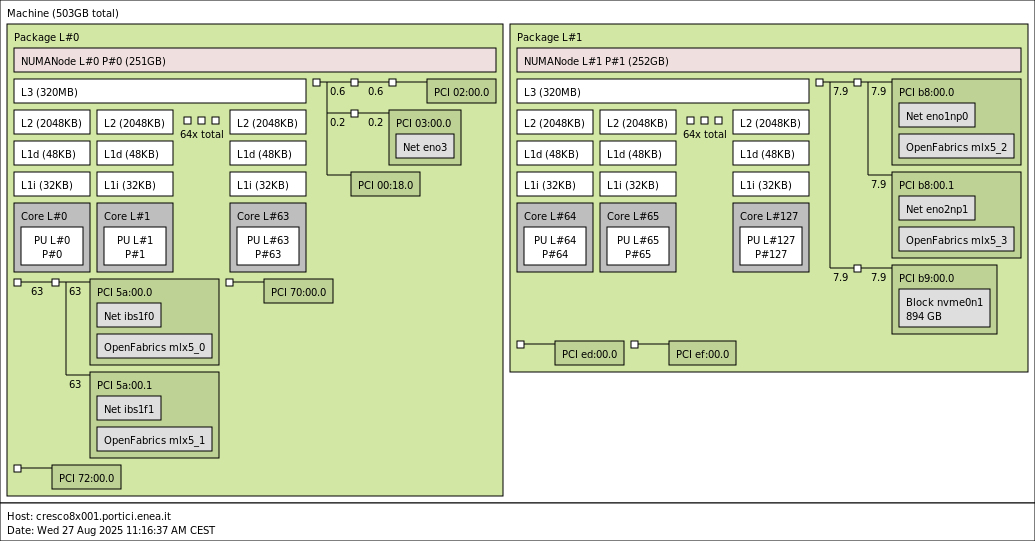
\includegraphics[width=\textwidth]{cresco8-cpu-node-diagram.png}
\caption{Topology of a CRESCO8 compute node as reported by
\texttt{lstopo}, captured on \texttt{cresco8x001.portici.enea.it}.  Two
packages, 64 cores each, with their own memory and network devices.  The
absence of memory-only NUMA nodes identifies this as a node of the
general CPU partition; an HBM node in Flat mode would show them.}
\label{fig:cresco8-lstopo}
\end{figure}

The manifest should be extended, subject to permissions, with the
following evidence:

\begin{table}[htbp]
\centering
\small
\tabsetup
\caption{Minimum platform record for an inference result.}
\label{tab:platform-record}
\begin{tabularx}{\textwidth}{@{}lY@{}}
\toprule
\headrow
\textbf{Category} & \textbf{Record} \\
\midrule
Identity
 & Hostname, Slurm job ID, partition, date and node allocation. \\
Processor
 & Exact SKU, sockets, physical cores, SMT state, microcode, governor,
   turbo policy and observed frequency. \\
Memory
 & Memory and clustering modes, NUMA distance matrix, HBM and DDR
   node IDs, DIMM population, huge-page state and measured local/remote
   bandwidth. \\
I/O
 & Lustre mount and striping used for model loading; NIC identity and
   NUMA affinity if multi-node tests are attempted. \\
Software
 & OS and kernel, loaded modules, compiler, runtime commit, linked
   libraries, build flags and complete command line. \\
Telemetry
 & Available RAPL, performance-counter and management-controller
   interfaces, including permissions and measurement boundaries. \\
\bottomrule
\end{tabularx}
\end{table}

This separation between documented configuration and observed
configuration is important.  Vendor documents establish what the platform \emph{can} support, and
ENEAGRID describes a dated cluster state.  \textbf{Only the archived
manifest establishes the conditions under which a reported result was
actually obtained.}


\clearpage
\part{Workload model and research evidence}
%======================================================================
%  Workload concepts and analytical model
%======================================================================

\section{A performance model for LLM inference}
\label{sec:inference-model}

\subsection{Prefill and autoregressive decode}

Inference for a decoder-only transformer has two phases
~\cite{na2024llmcpu}.  During
\emph{prefill}, the model processes the prompt and constructs the
initial key--value (KV) cache.  Tokens from the prompt can be processed
in parallel, so the linear layers often form comparatively large matrix
multiplications.  During \emph{decode}, the model generates one new
token per sequence at each iteration.  Each iteration requires the
relevant weights and KV state, then appends the key and value for the new
token.  Dense full-context attention reads the prior cached KV; sliding
window or sparse attention can reduce that history.
\figref{fig:prefill-decode} shows the two phases and the metric that
characterises each.

\begin{figure}[htbp]
\centering
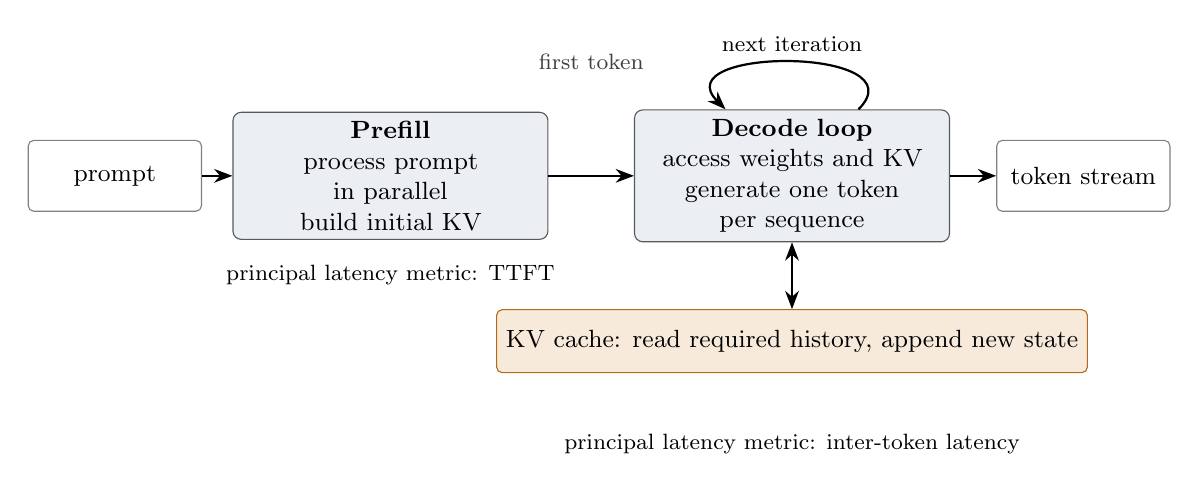
\begin{tikzpicture}[
  font=\small,
  io/.style={draw=black!50, fill=white, rounded corners=2pt,
             minimum width=2.2cm, minimum height=0.9cm, align=center},
  phase/.style={draw=black!65, fill=neutralcol, rounded corners=3pt,
                minimum width=4.0cm, minimum height=1.55cm,
                text width=3.7cm, align=center},
  kv/.style={draw=hbmcol!85!black, fill=hbmcol!16, rounded corners=2pt,
             minimum width=4.0cm, minimum height=0.8cm, align=center},
  flow/.style={-{Stealth}, thick},
  note/.style={font=\footnotesize, align=center}
]
  \node[io] (prompt) at (-6.0,0) {prompt};
  \node[phase] (prefill) at (-2.5,0)
    {\textbf{Prefill}\\process prompt in parallel\\build initial KV};
  \node[phase] (decode) at (2.6,0)
    {\textbf{Decode loop}\\access weights and KV\\
     generate one token\\per sequence};
  \node[io] (output) at (6.3,0) {token stream};
  \node[kv] (cache) at (2.6,-2.1)
    {KV cache: read required history, append new state};

  \draw[flow] (prompt) -- (prefill);
  \draw[flow] (prefill) -- (decode);
  \node[note, black!75] at (0.05,1.45) {first token};
  \draw[flow] (decode) -- (output);
  \draw[flow, {Stealth}-{Stealth}] (decode) -- (cache);
  \draw[flow] (decode.45) .. controls +(0.8,0.8) and +(-0.8,0.8)
       .. (decode.135) node[midway, above, note]{next iteration};

  \node[note, below=0.2cm of prefill]
    {principal latency metric: TTFT};
  \node[note, below=0.65cm of cache]
    {principal latency metric: inter-token latency};
\end{tikzpicture}
\caption{Dataflow of prompt prefill and autoregressive decode.  The
frequent description of prefill as compute-bound and decode as
bandwidth-bound is a useful first-order model, not a universal property:
batch, context, precision and kernel implementation can change the
regime.  Author's synthesis.}
\label{fig:prefill-decode}
\end{figure}

This phase distinction is essential when evaluating HBM.  A single
end-to-end throughput number can hide a faster decode phase behind a
long prompt, or hide a prefill regression behind a long generation.
\textbf{TTFT and decode latency must therefore be reported
separately.}  Prefill
usually offers matrix--matrix parallelism, whereas low-batch decode is
closer to matrix--vector execution and repeatedly streams weights.
Larger batches increase weight reuse and can move decode toward
matrix-engine throughput; long contexts simultaneously increase KV
traffic.


\subsection{Working-set capacity}
\label{sec:working-set}

For a model with \(P\) parameters and a stored weight precision of
\(q_w\) bits, \eqnref{eq:weights} gives the first-order weight
footprint:

\begin{equation}
\label{eq:weights}
  M_W = P\frac{q_w}{8} + M_{\mathrm{format}},
\end{equation}
\eqcaption{Resident weight footprint.  The second term is the one that surprises people: it collects scales, zero-points, alignment and any prepacked copy the runtime builds, so a GGUF file of a given size does not occupy that size in memory.}

where \(M_{\mathrm{format}}\) includes scales, zero-points, alignment,
and any prepacked or duplicated representation created by the runtime.
The model file size is \emph{not} the resident weight footprint, and
treating the two as interchangeable is the commonest way to misjudge
whether a model fits a tier.

For \(B\) concurrent sequences, cached length \(S\), \(L\) transformer
layers, \(H_{\mathrm{KV}}\) KV heads, head dimension \(d_h\), and
\(q_{\mathrm{KV}}\) bits per cached element, \eqnref{eq:kv} gives the
KV footprint:

\begin{equation}
\label{eq:kv}
  M_{\mathrm{KV}} =
  2 B S L H_{\mathrm{KV}} d_h \frac{q_{\mathrm{KV}}}{8}.
\end{equation}
\eqcaption{Key--value cache footprint.  It grows linearly in both context length \(S\) and batch \(B\), which is why long prompts and concurrency are the two ways to leave a memory tier.}

The factor two accounts for keys and values.  Grouped-query and
multi-query attention reduce the KV footprint because
\(H_{\mathrm{KV}}\) is smaller than the number of query heads.  The
complete resident set is

\begin{equation}
\label{eq:live}
  M_{\mathrm{live}} =
  M_W + M_{\mathrm{KV}} + M_{\mathrm{activations}}
  + M_{\mathrm{workspace}} + M_{\mathrm{runtime}}.
\end{equation}
\eqcaption{The live set.  This, not the model file, is the quantity that must be compared against usable local HBM.}

This arithmetic identifies where capacity boundaries may occur, but the
boundary must use the OS-exposed NUMA capacity on the allocated node and
a measured safety margin.  The advertised 64\,GB per socket is not a
usable-allocation guarantee: system use, allocator fragmentation and
workspace consume part of it.  A node may expose roughly 128\,GB across
two sockets, but that capacity is not uniformly local; using it requires
a placement strategy that distributes data and execution deliberately.

Quantization changes both sides of the experiment.  Fewer bits reduce
weight capacity and memory traffic, potentially reducing the benefit of
HBM for a model that already fits.  At the same time, quantization can
move a larger model below the HBM capacity boundary and remove DDR or
remote traffic altogether.  Packing, dequantization and kernel coverage
prevent performance from scaling exactly with bit width.  Weight and KV
precision must therefore be reported separately.

\subsection{Arithmetic intensity and the Roofline bound}
\label{sec:roofline}

The Roofline model, stated as \eqnref{eq:roofline}, relates arithmetic
intensity \(I=F/D\), measured in FLOP/byte, to compute throughput and
memory bandwidth~\cite{williams2009roofline}:

\begin{equation}
\label{eq:roofline}
  P_{\mathrm{attainable}}
  \leq
  \min\!\left(P_{\mathrm{compute}},
              I B_{\mathrm{effective}}\right).
\end{equation}
\eqcaption{The Roofline bound.  Performance is capped by whichever runs out first, arithmetic or bandwidth; changing memory tier moves only the second term.}

\eqnref{eq:step} is the corresponding lower-bound model for a single
inference step:

\begin{equation}
\label{eq:step}
  T_{\mathrm{step}}
  \gtrsim
  \max\!\left(
      \frac{F_{\mathrm{step}}}{P_{\mathrm{effective}}},
      \frac{D_{\mathrm{step}}}{B_{\mathrm{effective}}}
  \right)
  + T_{\mathrm{communication}} + T_{\mathrm{runtime}}.
\end{equation}
\eqcaption{Lower bound on one inference step.  The two trailing terms are the reason a measured speedup can fall well short of a bandwidth ratio even when the step really is memory-bound.}

The effective quantities must be measured for the selected kernel,
placement and core count.  Processor peak FLOP/s and theoretical pin
bandwidth are ceilings, not values to substitute uncritically.

For a dense linear layer during decode, if a stored weight is used once
for each of \(B\) sequences in a batch, \eqnref{eq:intensity} is a
useful first-order approximation:

\begin{equation}
\label{eq:intensity}
  I_{\mathrm{weights}} \approx \frac{2B}{b_w}
  \quad \text{FLOP/byte},
\end{equation}
\eqcaption{Arithmetic intensity of weight streaming in decode.  Batch size is in the numerator and bytes per weight in the denominator, so batching moves right along the Roofline and quantization moves right as well, both away from the region where a memory tier decides the outcome.}

where \(b_w\) is the stored bytes per weight and a multiply--add is
counted as two FLOPs.  The approximation assumes that each fetched dense
weight is reused across the \(B\) sequences.  At batch one, BF16 weight
streaming is therefore close to one FLOP/byte before KV,
activation and runtime traffic are included.  Batching reuses weights
and raises arithmetic intensity, which explains why HBM is expected to
matter most for low-batch decode and why AMX can become more important
as the matrix dimensions grow.

\figref{fig:roofline} makes the consequence visible.  Placing both
memory tiers on the same Roofline separates the region where a placement
decision can matter from the region where it cannot: to the left of the
ridge points the vertical distance between the two roofs is the full
bandwidth ratio, while to the right both roofs lie above the compute
ceiling, so no placement policy changes the bound.  Low-batch decode
sits in the first region and prefill in the second.  That is the
argument of this thesis expressed as a picture, and it is also why the
two phases have to be measured separately rather than folded into a
single throughput figure.

\begin{figure}[htbp]
\centering
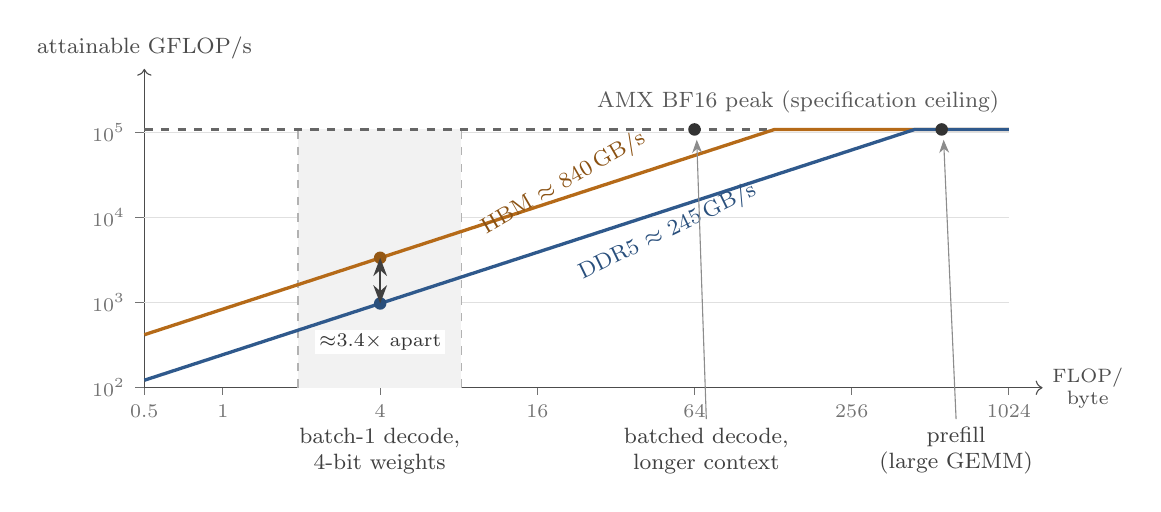
\begin{tikzpicture}[
  font=\small, x=1.22cm, y=1.0cm,
  roof/.style={very thick},
  point/.style={circle, fill=black!80, inner sep=1.6pt},
  lbl/.style={font=\footnotesize, align=center}
]
  \draw[->, black!70] (0,0) -- (9.35,0)
    node[right, font=\scriptsize, align=center]
      {FLOP/\\byte};
  \draw[->, black!70] (0,0) -- (0,4.05)
    node[above, font=\footnotesize] {attainable GFLOP/s};

  \foreach \X/\lab in {0/0.5, 0.818/1, 2.455/4, 4.091/16,
                       5.727/64, 7.364/256, 9.0/1024}
    \draw[black!55] (\X,0) -- (\X,-0.09) node[below, font=\scriptsize] {\lab};

  \foreach \Y/\lab in {0/{10^2}, 1.08/{10^3}, 2.16/{10^4}, 3.24/{10^5}}
    \draw[black!55] (0,\Y) -- (-0.10,\Y)
      node[left, font=\scriptsize] {$\lab$};

  \draw[black!12] (0,1.08) -- (9,1.08);
  \draw[black!12] (0,2.16) -- (9,2.16);
  \draw[black!12] (0,3.24) -- (9,3.24);

  \fill[black!5] (1.6,0) rectangle (3.3,3.28);
  \draw[black!30, dashed] (1.6,0) -- (1.6,3.28);
  \draw[black!30, dashed] (3.3,0) -- (3.3,3.28);

  \draw[dashed, thick, black!60] (0,3.28) -- (9,3.28);
  \node[lbl, black!65, anchor=south east] at (9,3.36)
    {AMX BF16 peak (specification ceiling)};

  \draw[roof, hbmcol!85!black] (0,0.673) -- (6.56,3.28) -- (9,3.28);
  \node[lbl, hbmcol!65!black, rotate=30, anchor=south west]
    at (3.55,1.72) {HBM $\approx$ 840\,GB/s};

  \draw[roof, ddrcol!85!black] (0,0.095) -- (8.02,3.28) -- (9,3.28);
  \node[lbl, ddrcol!75!black, rotate=26, anchor=north west]
    at (4.35,1.62) {DDR5 $\approx$ 245\,GB/s};

  \node[point, hbmcol!70!black] at (2.455,1.65) {};
  \node[point, ddrcol!75!black] at (2.455,1.07) {};
  \draw[{Stealth}-{Stealth}, thick, black!75] (2.455,1.07) -- (2.455,1.65);
  \node[font=\scriptsize, align=center, black!80, fill=white,
        inner sep=1.5pt] at (2.455,0.58) {$\approx$3.4$\times$ apart};

  \node[lbl, black!75] at (2.45,-0.80)
    {batch-1 decode,\\4-bit weights};
  \node[lbl, black!75] at (5.85,-0.80)
    {batched decode,\\longer context};
  \node[lbl, black!75] at (8.45,-0.80) {prefill\\(large GEMM)};

  \node[point] at (5.727,3.28) {};
  \node[point] at (8.30,3.28) {};
  \draw[black!45, -{Stealth}] (5.85,-0.40) -- (5.75,3.15);
  \draw[black!45, -{Stealth}] (8.45,-0.40) -- (8.32,3.15);

\end{tikzpicture}
\caption{Both memory tiers of one Xeon Max socket on a single Roofline.
The bandwidth figures are full-socket Flat-mode STREAM Triad values
measured on a Xeon Max 9470C~\cite{ibeid2025aurora} and are used only to
set the slopes; the compute ceiling is a specification figure rather
than a measurement, and neither has yet been established for CRESCO8.
The shaded band marks the operating region this thesis investigates:
left of the ridge points the vertical distance between the roofs is the
full bandwidth ratio, while past them both roofs coincide with the
compute ceiling and placement cannot move the bound.  Author's
synthesis.}
\label{fig:roofline}
\end{figure}


This model also clarifies why bandwidth alone is insufficient:

\begin{itemize}
  \item \textbf{Bandwidth} sets the rate for many concurrent,
        sufficiently regular memory requests.
  \item \textbf{Latency} sets the cost of a dependent or lightly loaded
        access path.  HBM can have higher unloaded latency than DDR5
        while sustaining much greater bandwidth under load
        ~\cite{ibeid2025aurora}.
  \item \textbf{Capacity} determines whether the critical working set
        remains local.  Crossing a 64\,GB socket boundary can introduce
        DDR5 or UPI traffic and cause a discontinuity that a simple
        single-tier Roofline does not predict.
\end{itemize}

For concurrent HBM and DDR5 traffic, a no-contention service-time
estimate can range from perfect overlap to serialization of the
per-tier transfers.  It is not a general bound: shared uncore resources,
cache conflicts, UPI traffic and memory-controller interference can make
the measured time worse than the serialized estimate.  Simultaneous
HBM--DDR traffic must therefore be characterized before a tiered
placement policy is modelled.

\subsection{Placement is part of the algorithm}

In Flat mode the operating system exposes memory tiers through NUMA,
but it does not know which model objects are bandwidth-critical.
Several mechanisms can therefore produce the wrong placement:
allocator first touch, worker migration, memory-mapped model pages,
automatic NUMA balancing, and a runtime that creates prepacked copies
after the initial allocation.  A command-line memory policy is evidence
of intent, \textbf{not evidence of residency}.

The relevant experimental object is consequently not ``the model in
HBM'' but a verified mapping between:

\begin{itemize}
  \item worker threads and physical cores;
  \item weight, KV, activation and workspace pages and their NUMA nodes;
  \item local or remote memory traffic observed during each inference
        phase; and
  \item the time interval used for performance and energy measurement.
\end{itemize}

This mapping is also the basis for testing topology-aware execution.
Independent replicas can use one local socket each; a single model can
be sharded across sockets or SNC domains; and selected objects can be
placed in different memory tiers.  These designs answer different
questions and should not be grouped under a generic ``two-socket run''.

\subsection{What we measure, and what each number means}
\label{sec:metrics}

A run of the experiment produces three kinds of number, and the most
common way to make a memory-placement study unreadable is to mix them.
A \textbf{result} is a quantity the thesis is willing to defend as an
outcome.  An \textbf{explanation} is a quantity that says \emph{why}
the outcome came out that way, and carries no weight on its own.  A
\textbf{validity check} is a quantity that decides whether the run
counts at all.  The tables below keep them apart, and every reported
comparison is expected to carry all three.

\subsubsection{Numbers that are results}

{\small\tabsetup
\begin{xltabular}{\textwidth}{@{}P{2.6cm}P{4.1cm}Y@{}}
\caption{Performance metrics: the quantities a claim may be made about.
A metric whose movement cannot be interpreted is not worth collecting,
so the right-hand column is the one to read first.}
\label{tab:metrics-results}\\
\toprule
\headrow
\textbf{Metric} & \textbf{What it is} & \textbf{Why it is here, and how to read it} \\
\midrule
\endfirsthead
\multicolumn{3}{@{}l}{\footnotesize\itshape Table~\ref{tab:metrics-results}, continued}\\[2pt]
\toprule
\headrow
\textbf{Metric} & \textbf{What it is} & \textbf{Why it is here, and how to read it} \\
\midrule
\endhead
\midrule
\multicolumn{3}{r@{}}{\footnotesize\itshape continued on the next page}\\
\endfoot
\bottomrule
\endlastfoot
\textbf{TTFT}\newline{\footnotesize time to first token}
& Elapsed time from an accepted request to the first emitted token.
& The visible cost of \emph{prefill}, and the only phase metric a long
  generation cannot hide.  \emph{Reading it:} scales with prompt
  length.  Because prefill sits right of the ridge point in
  \figref{fig:roofline}, a \textbf{large} tier effect here would be
  surprising and would need explaining. \\
\addlinespace[2pt]
\textbf{ITL}\newline{\footnotesize inter-token latency}
& The gap between consecutive emitted tokens, recorded per token.
& The decode metric, and where \(H_{1a}\) predicts the HBM effect will
  appear.  \emph{Reading it:} report the \textbf{distribution}
  (median, p95, p99), never a bare mean.  A stable median with a heavy
  tail points to allocation or scheduling interference, not to memory
  bandwidth. \\
\addlinespace[2pt]
\textbf{TPOT}\newline{\footnotesize time per output token}
& Mean decode time,
  \((T_{\mathrm{E2E}} - T_{\mathrm{TTFT}})/(O-1)\).
& A single summary of decode, and the metric the closest competing work
  reports~\cite{zhang2026cacheresident}.  \emph{Reading it:} good for
  comparison against published numbers, but it hides variance by
  construction, so it never appears without the ITL distribution beside
  it. \\
\addlinespace[2pt]
\textbf{Decode throughput}
& Output tokens per second, per sequence and aggregated over the batch.
& The form most readers expect and most CPU-inference papers publish.
  \emph{Reading it:} the reciprocal of TPOT, carrying no information
  TPOT does not; reported for comparability rather than for analysis. \\
\addlinespace[2pt]
\textbf{Prefill throughput}
& Prompt tokens per second, \(S/T_{\mathrm{TTFT}}\).
& Separates processing rate from prompt length, keeping runs with
  different prompts comparable.  \emph{Reading it:} roughly flat in
  prompt length once the prompt is long enough to fill the matrix
  units; a fall-off indicates a capacity or kernel effect. \\
\addlinespace[2pt]
\textbf{Tier ratio}\newline{\footnotesize \(R_{\text{phase}}\)}
& Per-phase ratio of matched DDR and HBM timings, \eqnref{eq:ratio}.
& \textbf{The headline result of the thesis.}  Everything else exists
  to make this number interpretable.  \emph{Reading it:}
  \(R_{\text{decode}} > R_{\text{prefill}}\) supports \(H_{1a}\); a
  \(R_{\text{decode}}\) below the STREAM bandwidth ratio supports
  \(H_{1b}\).  A value near \(1.0\) is \emph{a real finding}, not a
  failed experiment. \\
\end{xltabular}}


The tier ratio is defined on matched runs that differ in nothing but
placement:

\begin{equation}
\label{eq:ratio}
  R_{\text{phase}} =
  \frac{T_{\text{phase}}^{\text{DDR}}}{T_{\text{phase}}^{\text{HBM}}},
  \qquad \text{phase} \in \{\text{prefill}, \text{decode}\}.
\end{equation}
\eqcaption{Per-phase speedup from placing the live set in local HBM
rather than local DDR5.  Values above one mean HBM is faster.  Stated
per phase because a single end-to-end ratio would average the two
regimes of \figref{fig:roofline} into a number that describes neither.}

\subsubsection{Numbers that explain a result}

\tabref{tab:metrics-explain} lists the measurements that give a
result its mechanism.  The second row is the one to reach for first
when an effect turns out smaller than expected.


{\small\tabsetup
\begin{xltabular}{\textwidth}{@{}P{2.6cm}P{4.1cm}Y@{}}
\caption{Explanatory measurements.  None of these is a performance
claim.  Their job is to say why the numbers in
\tabref{tab:metrics-results} came out as they did, and, when the effect
is small, to separate \emph{the tier does not matter} from \emph{the
program never used the tier}.}
\label{tab:metrics-explain}\\
\toprule
\headrow
\textbf{Measurement} & \textbf{What it is} & \textbf{Why it is here, and how to read it} \\
\midrule
\endfirsthead
\multicolumn{3}{@{}l}{\footnotesize\itshape Table~\ref{tab:metrics-explain}, continued}\\[2pt]
\toprule
\headrow
\textbf{Measurement} & \textbf{What it is} & \textbf{Why it is here, and how to read it} \\
\midrule
\endhead
\midrule
\multicolumn{3}{r@{}}{\footnotesize\itshape continued on the next page}\\
\endfoot
\bottomrule
\endlastfoot
\textbf{Achieved bandwidth}
& Bytes per second actually moved to and from each tier during a phase,
  taken from memory-controller counters.
& \textbf{The most important explanatory number in the study};
  without it a null result cannot be diagnosed at all.
  \emph{Reading it:} compare against the STREAM figure measured on the
  same node, never against a published one. \\
\addlinespace[2pt]
\textbf{Bandwidth utilisation}
& Achieved bandwidth as a fraction of measured STREAM,
  \eqnref{eq:utilisation}.
& Turns the argument of \secref{sec:littles-law} into a measurement.
  \emph{Reading it:} a high tier ratio with high utilisation means the
  tier was the limit; a low tier ratio with \textbf{low} utilisation
  means \emph{concurrency} was the limit and the tier never got a
  chance. \\
\addlinespace[2pt]
\textbf{Remote traffic}
& Bytes crossing UPI to the other socket.
& The primary comparison is defined on one socket, so remote traffic
  means it was not.  \emph{Reading it:} expected near zero; anything
  else is a placement failure, and the run is re-examined rather than
  reported. \\
\addlinespace[2pt]
\textbf{Peak resident set}
& Maximum resident memory, decomposed into weights, KV state and
  workspace per \eqnref{eq:live}.
& Locates the capacity boundary the second research question is about.
  \emph{Reading it:} compared against \emph{usable} local HBM on the
  allocated node, which is smaller than the nominal 64\,GB. \\
\addlinespace[2pt]
\textbf{Frequency and power}
& Sustained socket clock, package power and throttling state over the
  measured interval.
& Guards against reporting a thermal effect as a placement effect.
  \emph{Reading it:} must be equivalent across the two placements being
  compared; if it is not, the comparison is confounded. \\
\end{xltabular}}


\begin{equation}
\label{eq:utilisation}
  U_{\text{tier}} =
  \frac{B_{\text{achieved}}}{B_{\text{STREAM}}} .
\end{equation}
\eqcaption{Bandwidth utilisation: the fraction of a tier's measured
sustainable bandwidth that the workload actually drew.  This is the
number that decides how a disappointing tier ratio should be read.  A
decode phase running at \(U_{\mathrm{HBM}} \approx 0.3\) has not shown
that HBM fails to help; it has shown that the workload asked HBM for
nothing DDR5 could not also have supplied.}

\subsubsection{Numbers that decide whether a run counts}

The checks in \tabref{tab:metrics-validity} come first in the analysis,
not last.  A run that fails any of them is discarded before its timings
are looked at, because a placement study whose placement was not
verified is not evidence of anything.

{\small\tabsetup
\begin{xltabular}{\textwidth}{@{}P{2.55cm}YP{4.3cm}@{}}
\caption{Validity checks applied to every run before its results are
considered.  These are pass/fail, not quantities to be reported as
findings.}
\label{tab:metrics-validity}\\
\toprule
\headrow
\textbf{Check} & \textbf{What it establishes} &
\textbf{Passing condition} \\
\midrule
\endfirsthead
\multicolumn{3}{@{}l}{\footnotesize\itshape Table~\ref{tab:metrics-validity}, continued}\\[2pt]
\toprule
\headrow
\textbf{Check} & \textbf{What it establishes} &
\textbf{Passing condition} \\
\midrule
\endhead
\midrule
\multicolumn{3}{r@{}}{\footnotesize\itshape continued on the next page}\\
\endfoot
\bottomrule
\endlastfoot
\textbf{Page residency}
& That the live set is where the command line said it should be.  A
  memory policy states an intention; only a page count states an
  outcome.
& The overwhelming majority of the process's resident pages sit on the
  intended NUMA node, with the threshold fixed before the campaign and
  the shortfall reported. \\
\addlinespace[1pt]
\textbf{Thread binding}
& That the cores executing the work are local to the memory holding it.
& Observed CPU affinity matches the requested binding for every worker
  thread. \\
\addlinespace[1pt]
\textbf{Output equivalence}
& That placement changed the speed and nothing else.
& For a fixed seed and identical inputs, the generated token sequence
  is identical across tiers.  A divergence indicates a defect, not a
  finding. \\
\addlinespace[1pt]
\textbf{Repetition dispersion}
& That an observed difference is larger than the noise it sits in.
& Coefficient of variation across repetitions small enough that the
  tier effect exceeds it; repetitions, warm-up and discarded runs all
  reported. \\
\addlinespace[1pt]
\textbf{Thermal state}
& That the node was in a comparable operating condition for both arms.
& No throttling events, and equivalent sustained frequency across the
  compared placements. \\
\end{xltabular}}


\subsubsection{Where each timing starts and stops}

The two phase metrics compose, as \eqnref{eq:e2e} shows, into the
latency a user actually experiences over \(O\) generated tokens in one
synchronous request:

\begin{equation}
\label{eq:e2e}
  T_{\mathrm{E2E}}
  =
  T_{\mathrm{TTFT}} +
  \sum_{j=2}^{O} T_{\mathrm{ITL},j}.
\end{equation}
\eqcaption{End-to-end request latency as the sum of its two phases.
Written this way to make the risk explicit: a single end-to-end figure
can absorb a decode improvement into a long prompt, or a prefill
regression into a long generation, which is why this thesis reports the
two terms rather than their sum.}

A latency figure is meaningless without its boundary, and boundaries
differ enough between published studies that comparing numbers across
papers is often comparing definitions~\cite{agrawal2025evaluating}.
This thesis fixes them as follows.  Model loading, tokenizer
construction and the first warm-up request lie \emph{outside} every
reported timing.  TTFT starts when the prompt has been tokenized and
submitted, and stops when the first token is available.  ITL is
measured between token emissions and excludes detokenization of the
final output.  Every reported figure comes from a warmed process, and
the number of discarded warm-up iterations is recorded with the run.

Two further distinctions are worth stating because they are routinely
elided.  Static batch throughput and online serving goodput are
different constructs: the second depends on an arrival process, a
scheduler and a declared latency objective, none of which are part of
this study.  And hardware counters are explanatory measurements rather
than performance metrics.  Their collection overhead, multiplexing
behaviour and measurement scope are documented alongside the values, or
the values are not used.

\subsection{Predictions to test}

The model yields three bounded predictions:

\begin{enumerate}
  \item local HBM should benefit low-batch decode more than compute-dense
        prefill, but the speedup need not equal the STREAM bandwidth
        ratio;
  \item performance should change when the verified live set crosses a
        local HBM boundary, with the size and direction of the change
        depending on placement and memory mode; and
  \item batching and lower-bit weights should reduce weight-bandwidth
        pressure, while long contexts can reintroduce pressure through
        the KV cache.
\end{enumerate}

These statements are hypotheses.  The literature reviewed next
motivates them but does not establish them for CRESCO8.

%======================================================================
%  Literature review: the state of the art
%======================================================================

\section{The state of the art}
\label{sec:literature}

Two bodies of work bear on this thesis, and they have grown up almost
independently of each other.  One asks whether a general-purpose CPU can
run a language model quickly enough to be worth using, and answers it by
rewriting arithmetic: quantized weights, cheaper kernels, better use of
the matrix units.  The other asks how much performance depends on
\emph{where} data sits in a tiered memory system, and answers it with
placement experiments, historically on HPC codes and more recently on
the key--value cache of a transformer.  Each line is mature.  \textbf{Their intersection, on a CPU that
actually has two memory tiers under software control, is close to
empty}, and that emptiness is what this thesis is built on.

\subsection{Scope of the review}

The review covers three bodies of work, chosen because each constrains
the study in a different way.  The first is the line of research that
made CPU inference practical through quantization, kernel design and use
of the matrix units.  It supplies the performance figures any result
here will be read against.  The second is work on \emph{memory tiering},
in high-performance computing where it is mature and in transformer
inference where it is not, which supplies the mechanism this thesis
tests.  The third is the smaller methodological literature on evaluating
inference systems, which constrains how the measurements must be taken
and reported.

Two boundaries are worth stating.  Work on training, on distributed
serving and on accelerator microarchitecture is excluded: it is a large
literature, and none of it bears on a single-socket placement question.
And a number of the works discussed below are preprints rather than
refereed publications.  They are cited where they establish what the
field is currently attempting, and their status is noted where a
quantitative claim rests on them, since an unrefereed number is a weaker
foundation than a refereed one.

\secref{sec:related-work} then departs from this survey and reads four
sources closely, on the grounds that they alone were measured on the
processor family studied here.

\subsection{Making the CPU a credible inference target}
\label{sec:lit-arithmetic}

CPU inference became a serious proposition when weight-only quantization
was combined with kernels written for it.  Shen et al.\ paired an
automatic INT4 flow with a purpose-built runtime and reported 20--80\,ms
per generated token for 6--20\,B models on a single fourth-generation
Xeon socket, within a percent of FP32 accuracy~\cite{shen2023efficientcpu}.
The significance is less the latency than the demonstration that the
gap to an accelerator was a software gap as much as a hardware one.

In practice most CPU inference now happens through
\lcpp{}~\cite{llamacpp2026}, the runtime adopted here, and the published
measurements of it provide a useful calibration.  Malakhov benchmarks seven 4-bit GGUF
models across three CPU environments, including a Xeon Platinum 8592+,
reporting roughly 120 tokens/s for a 1\,B model, 45 for a 7\,B model and
15 for a 24\,B model~\cite{malakhov2025medlocalgpt}.  That machine is
the DDR-only sibling of the processor studied here, being the same
generation with a comparable core count and no on-package HBM.  That
makes it the closest thing in the literature to a published control for the comparison in
\secref{sec:research-gap}.  Kurt supplies the orthogonal sweep,
evaluating 3- to 8-bit K-quant and legacy GGUF formats on one model for
accuracy, perplexity and CPU prefill and decode throughput together,
which is the evidence needed to choose a quantization level on grounds
other than habit~\cite{kurt2026quantization}.

Alongside the runtimes sits a line of work on the kernels themselves,
unified by the observation that a quantized matrix--vector product
spends most of its time on operations the hardware is bad at.  Zhang et
al.\ replace multiply--accumulate in attention with in-register SIMD
lookups and roughly double the speed of a 4-bit LLaMA-7B at 16\,k
context~\cite{zhang2024nomad}.  Wei et al.\ generalise the idea to the
weight path, computing mixed-precision GEMM by table lookup with no
dequantization step at all, and report up to 4$\times$ over \lcpp{}
together with a 70\% reduction in energy~\cite{wei2025tmac}.  Zuo et
al.\ push furthest, fusing eight sub-GEMVs of a ternary layer into a
single AVX-512 loop of masked additions and subtractions, with no
multiplications anywhere in the inner
loop~\cite{zuo2026fairyfuse}.

\begin{table}[htbp]
\centering
\small
\tabsetup
\caption{Arithmetic-side work on CPU inference.  Reported gains are
against the baseline named in each paper and on that paper's hardware;
they are not mutually comparable, and are listed to show the shape of
the field rather than to rank it.}
\label{tab:lit-arithmetic}
\begin{tabularx}{\textwidth}{@{}P{2.5cm}P{3.1cm}YP{3.1cm}@{}}
\toprule
\headrow
\textbf{Work} & \textbf{Platform} & \textbf{Lever} &
\textbf{Baseline and gain} \\
\midrule
Shen et al.\ 2023~\cite{shen2023efficientcpu}
& 4th-gen Xeon, one socket
& INT4 weight-only quantization with a matched runtime
& 20--80\,ms/token for 6--20\,B; \(\leq\)1\% accuracy loss vs FP32 \\
\addlinespace[2pt]
Zhang et al.\ 2024~\cite{zhang2024nomad}
& x86 with SIMD registers
& Attention by in-register lookup instead of multiply--add
& \(\approx\)2$\times$ on 4-bit LLaMA-7B at 16\,k context \\
\addlinespace[2pt]
Wei et al.\ 2025~\cite{wei2025tmac}
& Apple M2-Ultra, Raspberry Pi 5
& Table-lookup mixed-precision GEMM, no dequantization
& Up to 4$\times$ over \lcpp{}; 70\% less energy \\
\addlinespace[2pt]
Zuo et al.\ 2026~\cite{zuo2026fairyfuse}
& Intel Xeon 8558P
& Ternary weights, eight sub-GEMVs fused into one AVX-512 loop
& 29.6$\times$ at kernel level; \textbf{1.24$\times$ end to end} over
  \lcpp{} Q4\_K\_M \\
\bottomrule
\end{tabularx}
\end{table}

\subsection{Where the arithmetic-side lever runs out}
\label{sec:lit-pivot}

The last row of \tabref{tab:lit-arithmetic} is the most informative
number in this section, and it is worth dwelling on.  Zuo et al.\ make
their kernel almost thirty times faster and the model runs 1.24 times
faster.  Nothing went wrong in their engineering: \emph{the arithmetic simply
stopped being what the program was waiting for}.  Once a phase spends
most of its time waiting for weights to arrive, removing instructions
from that phase buys very little, and the marginal return on further
kernel work collapses.

This is the pivot on which the rest of the review turns.  A decade of
effort has moved CPU inference from implausible to routine by making the
work cheaper, and that effort has been successful enough to expose what
lies underneath it.  The interesting question is no longer how few
operations a token can be generated with, but how quickly the bytes
those operations consume can be delivered, which is a question about the
memory system and therefore about placement.
\figref{fig:two-levers} sets the two lines of attack against each other
and marks the point at which they stop being interchangeable.

\begin{figure}[htbp]
\centering
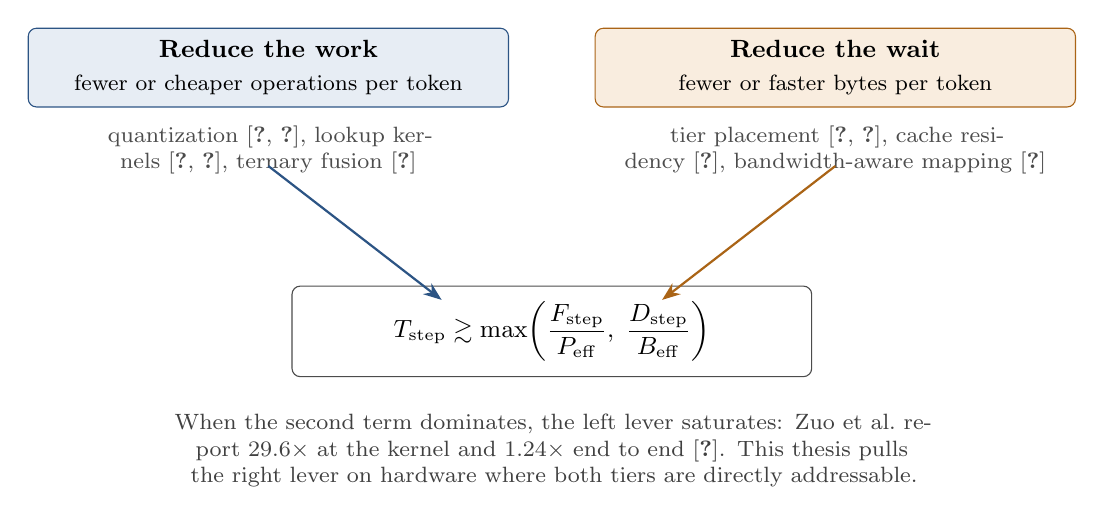
\begin{tikzpicture}[
  font=\small,
  lever/.style={draw=black!65, fill=neutralcol, rounded corners=3pt,
                minimum width=6.1cm, minimum height=1.0cm, align=center},
  work/.style={font=\footnotesize, text width=5.9cm, align=center,
               inner sep=2pt},
  target/.style={draw=black!70, fill=white, rounded corners=3pt,
                 minimum width=6.6cm, minimum height=1.15cm,
                 align=center},
  arr/.style={-{Stealth}, thick, black!60}
]
  \node[lever, fill=ddrcol!12, draw=ddrcol!80!black] (a) at (-3.6,2.6)
    {\textbf{Reduce the work}\\[1pt]
     \footnotesize fewer or cheaper operations per token};
  \node[work, below=0.15cm of a, text=black!70]
    {quantization~\cite{shen2023efficientcpu,kurt2026quantization},
     lookup kernels~\cite{zhang2024nomad,wei2025tmac},
     ternary fusion~\cite{zuo2026fairyfuse}};

  \node[lever, fill=hbmcol!14, draw=hbmcol!80!black] (b) at (3.6,2.6)
    {\textbf{Reduce the wait}\\[1pt]
     \footnotesize fewer or faster bytes per token};
  \node[work, below=0.15cm of b, text=black!70]
    {tier placement~\cite{fang2025kvplacement,jang2026itme},
     cache residency~\cite{zhang2026cacheresident},
     bandwidth-aware mapping~\cite{lu2026thinfer}};

  \node[target] (t) at (0,-0.75)
    {\(T_{\mathrm{step}} \gtrsim
       \max\!\left(\dfrac{F_{\mathrm{step}}}{P_{\mathrm{eff}}},\;
                   \dfrac{D_{\mathrm{step}}}{B_{\mathrm{eff}}}\right)\)};

  \draw[arr, ddrcol!80!black] (-3.6,1.35) -- (-1.4,-0.35);
  \draw[arr, hbmcol!80!black] (3.6,1.35) -- (1.4,-0.35);

  \node[font=\footnotesize, text width=11.4cm, align=center,
        below=0.35cm of t, text=black!75]
    {When the second term dominates, the left lever saturates: Zuo et
     al.\ report 29.6$\times$ at the kernel and 1.24$\times$ end to
     end~\cite{zuo2026fairyfuse}.  This thesis pulls the right lever on
     hardware where both tiers are directly addressable.};
\end{tikzpicture}
\caption{The two ways of shortening a decode step, and the point at
which they stop being interchangeable.  Author's synthesis; the
lower-bound expression is the step model developed in
\secref{sec:roofline}.}
\label{fig:two-levers}
\end{figure}


\subsection{Moving the data instead}
\label{sec:lit-placement}

\subsubsection{What HPC already knows}

Tiered main memory is not new, and the HPC community learned most of the
relevant lessons on Knights Landing.  Peng et al.\ compared MCDRAM with
DRAM across scientific and analytics workloads and found a split that
has aged well: codes with regular access patterns gained up to
3$\times$, while codes with irregular patterns were latency-bound and
could run \emph{slower} in the high-bandwidth tier
alone~\cite{peng2017hybridmemory}.  Their remedy, more hardware threads to keep enough requests in flight
for the bandwidth to be reachable, is the same concurrency argument
developed in \secref{sec:littles-law}, and it is the most direct published
warning that a fast tier is not automatically a faster program.

On the processor used here, Reguly provides the closest non-LLM
reference point, reporting 2.0--4.3$\times$ over the previous generation
on bandwidth-sensitive HPC proxies and, importantly, observing that for
some codes the bottleneck moves from bandwidth to communication
latency once bandwidth stops being scarce~\cite{reguly2023xeonmax}.  That
observation is the reason this thesis does not expect an inference
speedup equal to the STREAM ratio, and it sets the scale against which a
smaller measured effect should be judged.

\subsubsection{Tiering for inference}

Applying the same idea to transformers is recent and, so far, mostly
indirect.  Fang et al.\ give the problem its formal treatment, casting
KV-cache placement across a fast and a slow tier as latency
minimisation and deriving an upper bound of up to 5.87$\times$ over
static placement~\cite{fang2025kvplacement}.  Three properties of that
work matter here.  It is evaluated in a behavioural simulator rather
than on hardware; it covers the decode stage only; and it fixes model
weights in the fast tier by assumption, on the grounds that weights are
read at every step, leaving KV entries as the only variable.  The last
of these is the assumption a Xeon Max socket is able to break, because
64\,GB of HBM, and only 16\,GB per domain under SNC4, is not comfortably
larger than a quantized model of interest.

Neighbouring systems work approaches the same architecture from other
directions.  Jang et al.\ exploit the predictable access pattern of
weights and prefix state to expand KV capacity across host DRAM,
CXL-attached memory and NVMe, reporting a 35.7\% throughput
improvement~\cite{jang2026itme}, and a companion design places a
three-tier stack behind a CXL interface for multi-turn
serving~\cite{jang2026hymcache}.  Most directly comparable to this
thesis, Zhang et al.\ keep reusable weights resident in a GB-scale
last-level cache on a multi-socket CPU, separating weight-centric
operators from attention and KV management, and report 2.04--11.51$\times$
on time per output token against \lcpp{} with equivalent
resources~\cite{zhang2026cacheresident}.  Their argument is this thesis's argument with a different fast tier:
\emph{SRAM instead of HBM, bought with a redesigned runtime rather than
with placement}.

\tabref{tab:lit-tiering} collects this work and makes the pattern
visible.  At larger scale, Lu et al.\ build an inference framework for
the MT-3000
many-core processor of the Tianhe supercomputer, framing the problem
explicitly as maximising locality under a bandwidth constraint and
beating DeepSpeed on 2$\times$V100S by 62--73\% for a 7\,B
model~\cite{lu2026thinfer}.  Chen et al.\ show that the CPU side of a
hybrid deployment is itself the bottleneck, using AMX-specialised
kernels and asynchronous scheduling to obtain 4.62--19.74$\times$
prefill and 1.25--4.09$\times$ decode speedups on large
MoE models~\cite{chen2025ktransformers}; He et al.\ establish that
scaling CPU inference beyond one socket is ordinary
practice~\cite{he2024distributedcpu}.  Taken together these say that
CPU-side memory behaviour is worth improving even when a GPU is
present.

\begin{table}[htbp]
\centering
\small
\tabsetup
\caption{Placement and tiering work relevant to the questions in \secref{sec:research-gap}.  The
final column is the one that matters: almost all inference-side evidence
is simulated, accelerator-attached, or obtained by rebuilding the
runtime.}
\label{tab:lit-tiering}
\begin{tabularx}{\textwidth}{@{}P{2.45cm}P{3.3cm}YP{2.7cm}@{}}
\toprule
\headrow
\textbf{Work} & \textbf{Tiers} & \textbf{What is placed} &
\textbf{Evidence} \\
\midrule
Peng et al.\ 2017~\cite{peng2017hybridmemory}
& MCDRAM / DRAM, one socket
& Whole application; regular vs irregular access compared
& Measured, HPC codes \\
\addlinespace[2pt]
Reguly 2023~\cite{reguly2023xeonmax}
& HBM2e / DDR5, Xeon Max
& Whole application
& Measured, HPC proxies \\
\addlinespace[2pt]
Fang et al.\ 2025~\cite{fang2025kvplacement}
& GPU HBM3 / CPU LPDDR5X over NVLink-C2C
& KV entries only; weights pinned in HBM by assumption
& \textbf{Simulated}, decode only \\
\addlinespace[2pt]
Jang et al.\ 2026~\cite{jang2026itme}
& Host DRAM / CXL / NVMe
& Weights and prefix cache, by access predictability
& Measured, capacity expansion \\
\addlinespace[2pt]
Zhang et al.\ 2026~\cite{zhang2026cacheresident}
& LLC / DRAM, multi-socket CPU
& Weights held cache-resident; KV scaled separately
& Measured, \textbf{requires a redesigned runtime} \\
\addlinespace[2pt]
\textbf{This thesis}
& \textbf{HBM2e / DDR5, one Xeon Max socket}
& \textbf{Whole process first; then weights against KV state}
& \textbf{Measured, unmodified runtime, residency verified} \\
\bottomrule
\end{tabularx}
\end{table}


\subsection{Whether decode is bandwidth-bound, and why it might not be}
\label{sec:lit-bandwidth}

The claim that autoregressive decode is memory-bound is close to folklore
now, and it is usually justified with a roofline argument.  Yuan et al.\
supply the canonical version, building a survey of inference efficiency
on an explicit roofline analysis and showing why low-batch decode sits
far to the left of the ridge point~\cite{yuan2024roofline}.  Bi et al.\
turn the same model into a benchmarking framework and add a detail this
thesis needs: operational intensity is not a fixed property of a model
but moves with sequence length and depth~\cite{bi2026rooflinebench},
which is precisely the mechanism behind the capacity sweep in
\secref{sec:working-set}.

What the folklore leaves out is that being memory-bound and being
bandwidth-limited are different conditions, and only the second is cured
by a faster tier.  Chen reports a cross-GPU study of batch-1 decode in
which faster memory conspicuously fails to deliver proportional latency
gains: an L4 reaches 81\% of its peak bandwidth while an H100 reaches
27\%, and launch overhead and kernel choice matter more than the
bandwidth on the specification sheet~\cite{chen2026memorybound}.  The
work is GPU-side, so it transfers as a mechanism rather than as a
comparable measurement, but the mechanism is exactly the one that would
produce a disappointing HBM result here, and it is the strongest
published reason to state \(H_{1b}\), that the observed ratio will fall
short of the STREAM ratio, as a hypothesis rather than as a concession.

Arif et al.\ add a third regime.  Studying models from 8\,B to 671\,B on
GPU clusters, they describe reasoning-heavy workloads as
\emph{capacity-bound} rather than compute- or bandwidth-bound, and
identify KV-cache fragmentation as a mechanism that throttles
throughput before any bandwidth ceiling is
reached~\cite{arif2026inferencescaling}.  For this thesis that is both a
vocabulary and a warning: the transition
\secref{sec:research-gap} sets out to locate could be produced by
fragmentation rather than by tier capacity, and the two have to be told
apart.

\subsection{How the field measures, and how it gets it wrong}
\label{sec:lit-method}

A memory-placement result is a comparison, and comparisons of inference
systems are easy to draw badly.  Agrawal et al.\ catalogue the failure
modes across three axes: baselines that conflate engineering effort with
algorithmic novelty, workloads that do not resemble anything deployed,
and normalised metrics that conceal generation stalls.  They also supply
a checklist for avoiding them~\cite{agrawal2025evaluating}.
Their argument is the reason the comparison at the centre of this thesis
holds the build, thread count, model, quantization and prompt fixed and
varies only the memory tier, and the reason inter-token latency will be
reported as a distribution rather than as a mean.

Two further papers shape the protocol.  Salaria et al.\ propose metrics
for the cost of benchmarking itself and show that a well-chosen subset
of a sweep can retain most of its information.  Reducing generation
length from 1024 to 128 tokens preserved 96.6\% of the accuracy of the
full measurement at 2.7$\times$ less cost~\cite{salaria2025metametrics}.
On a shared allocation with a 24-hour limit that is not a convenience
but a design constraint, and it gives a defensible basis for a reduced
factor matrix instead of an arbitrary one.  Stuhlmann et al.\ report
latency, throughput, energy and startup time side by side across
engines and quantizations and conclude that no configuration wins
everywhere~\cite{stuhlmann2025bench360}; their results are GPU-side, but
the reporting structure is the right template for a results chapter
whose honest conclusion will also be conditional.

For placing CPU inference in a wider hardware context without expanding
the scope of the experiments, Li et al.\ provide a cross-platform survey
covering CPU, GPU, FPGA, ASIC and processing-in-memory designs, with
tokens per second and tokens per joule at small batch
sizes~\cite{li2024hardwareperspective}.

\subsection{Where this thesis sits}
\label{sec:lit-position}

Reading the two lines of work together produces a fairly sharp picture.
The arithmetic-side line has largely done its job and is now limited by
data movement.  The memory-side line has strong measured results in HPC,
where the object being placed is an array, and much weaker measured
results in inference, where the object being placed is a weight tensor
or a KV cache.  The inference-side tiering evidence is dominated by
simulation~\cite{fang2025kvplacement}, by accelerator-attached
hierarchies reached over an interconnect~\cite{jang2026itme,jang2026hymcache},
or by results that required rebuilding the runtime around a different
fast tier~\cite{zhang2026cacheresident}.

A Xeon Max socket is unusual in that it removes all three of those
qualifications at once.  Both tiers are directly load/store addressable
by the same cores, so placement is a page policy rather than a transfer;
the runtime does not have to be modified for the primary comparison; and
the fast tier is small enough relative to a quantized model that the
weights-fit assumption underlying the published formulation can be made
to fail on purpose.  What is missing from the literature, and what
\secref{sec:research-gap} sets out to supply, is the corresponding
measurement: a phase-resolved comparison of verified local-HBM and
local-DDR placement for quantized \lcpp{} inference, with page residency
and achieved bandwidth reported, on hardware rather than in a model.

Whether that measurement is the first of its kind is not a claim this
review makes.  The search described above was not systematic enough to
support it, and the more useful framing is in any case comparative: the
prediction exists, the bound has been derived, and what has not been
done is to hold it against a real machine.

%======================================================================
%  Close reading of the four Xeon Max sources, and the gap
%======================================================================

\section{Evidence measured on Xeon Max}
\label{sec:related-work}

\secref{sec:literature} surveyed a field; this section reads four
papers closely.  The distinction is deliberate.  Almost none of the work
discussed so far was measured on the processor studied here, and a
result obtained on an H100, an M2-Ultra or a behavioural simulator
\textbf{transfers as a mechanism, not as a number}.  Four sources do sit on or beside Xeon
Max hardware, and they are consequently the ones whose numbers could
plausibly be reproduced, contradicted or extended on CRESCO8.  It is
therefore worth establishing exactly what each of them measured, under
what conditions, and how far the result travels.

They divide the work between them.  Na et al.\ supply the closest
workload precedent, being the only one of the four to run a language
model on this processor~\cite{na2024llmcpu}.  Ibeid et al.\ isolate the
memory system itself, covering bandwidth, latency, mode and locality,
without an LLM in sight~\cite{ibeid2025aurora}.  Goto et al.\ show what
deliberate tier staging and resource mapping look like at production
scale~\cite{goto2026aurorahpl}.  Dongarra et al.\ supply the
architectural argument for why the question is worth asking at all, and
are treated as motivation rather than as a
baseline~\cite{dongarra2026gpus}.  Each carries a transfer limit, and
those limits are stated alongside the results rather than collected in a
caveat at the end.

\subsection{Na et al.: the closest inference precedent}
\label{sec:na-review}

Na et al.\ evaluate Intel Extension for PyTorch (IPEX) on a dual-socket
Xeon Max 9468 server and compare it with a previous-generation Xeon and
with single A100 and H100 GPUs running FlexGen
~\cite{na2024llmcpu}.  Their main comparisons bind one 48-core Max
socket; only the core-count sweep extends to 96 cores.  The CPU
experiments use BF16 OPT and LLaMA-2 models, prompt length 128,
generation length 32 and batch sizes from 1 to 32; a separate sweep
increases the prompt length.  This is the closest platform and workload
match in the corpus, but its results need careful qualification, which
\tabref{tab:na-findings} supplies claim by claim.

\begin{table}[htbp]
\centering
\small
\tabsetup
\caption{Results from Na et al.\ and the interpretation used here
~\cite{na2024llmcpu}.}
\label{tab:na-findings}
\begin{tabularx}{\textwidth}{@{}YYY@{}}
\toprule
\headrow
\textbf{Reported result} & \textbf{What it supports}
 & \textbf{What it does not establish} \\
\midrule
Depending on batch, Xeon Max geometric-mean throughput over the tested
models is 3.2--6.3$\times$ that of the Ice Lake system.
 & Matrix acceleration and the newer memory system make recent CPUs
   substantially more credible for inference.
 & A causal HBM or AMX speedup: cores, cache, DDR generation,
   microarchitecture and software paths also change. \\
\addlinespace[2pt]
Quadrant+Flat gives the best average of the four configurations under
the paper's HBM-first Flat placement.
 & In this setup, explicit HBM placement outperforms hardware-managed
   caching; unmanaged fine-grained NUMA is costly.
 & A universal preference for Quadrant mode.  Exact allocation,
   first-touch and binding details are not disclosed. \\
\addlinespace[2pt]
On average over the tested models and batches, 48 cores outperform a
naive 96-core execution.
 & Remote traffic can erase the value of additional cores.
 & An inherent one-socket scaling limit; replicas or topology-aware
   sharding are not evaluated. \\
\addlinespace[2pt]
At batch one, the CPU outperforms the tested FlexGen A100/H100 runs for
oversized models.
 & Capacity and data movement can dominate accelerator arithmetic at
   low batch.
 & General CPU superiority.  For LLaMA2-70B at batch 16 and prompt
   length at least 256, the offloaded H100 regains lower latency; when a
   model fits GPU memory, the GPUs are faster.  Multi-GPU serving is not
   tested. \\
\bottomrule
\end{tabularx}
\end{table}

The paper's GPU result is therefore best read as \textbf{a
data-movement result}, not as a verdict on CPUs against GPUs.
It compares direct CPU execution with a particular single-GPU
offloading system.  It does not compare like-for-like production
serving stacks.  The study also omits quantized weights, long
generations, energy, online arrivals, tail latency and output-quality
validation.  Repetition count, dispersion, complete software versions,
firmware, warm-up and the exact NUMA command are not reported.  Its
experimental design can be reimplemented, but the paper does not
support exact numerical reproduction.  It also proposes, without
implementing or evaluating, NUMA-aware hot/cold placement and
CPU--GPU layer partitioning.  A later placement contribution must
acknowledge that prior proposal.

\subsection{Ibeid et al.: bandwidth, latency and locality}
\label{sec:ibeid-review}

Ibeid et al.\ separate memory-system effects more clearly
~\cite{ibeid2025aurora}.  On the Borealis testbed they use Xeon Max
9470C processors and run STREAM, Intel Memory Latency Checker, PCIe and
MPI microbenchmarks, followed by three HPC applications chosen to stress
bandwidth, latency or capacity.  At the time of the study, production
Aurora was configured in Quadrant+Flat mode; the full single-socket
Flat/Cache and Quadrant/SNC4 matrix comes from Borealis, and the
bandwidth figures this thesis reuses are those in
\tabref{tab:ibeid-stream}.

\begin{table}[htbp]
\centering
\small
\tabsetup
\caption{Single-socket STREAM Triad bandwidth on the Borealis Xeon Max
9470C testbed, in GB/s~\cite{ibeid2025aurora}.  The paper does not fully
specify array size, first touch or cache-state controls.}
\label{tab:ibeid-stream}
\begin{tabular}{@{}lccc@{}}
\toprule
\headrow
 & \multicolumn{2}{c}{\textbf{Flat mode}} & \textbf{Cache mode} \\
\cmidrule(lr){2-3}
\textbf{Clustering} & \textbf{DDR5} & \textbf{HBM} & \textbf{DDR5+HBM cache} \\
\midrule
Quadrant, full socket & 235 & 680 & 560 \\
SNC4, full socket     & 245 & 840 & 575 \\
SNC4, one quadrant    &  60 & 210 & 150 \\
\bottomrule
\end{tabular}
\end{table}

In the two full-socket Flat-mode rows, HBM bandwidth is 2.9--3.4 times
DDR5 bandwidth, and SNC4 raises full-socket HBM bandwidth by about 24\%
over Quadrant.
However, unloaded latency favours DDR5: the paper reports 112.9\,ns for
Quadrant/DDR and 134.9\,ns for Quadrant/HBM.  Under increasing access
load, DDR5 saturates sooner while HBM sustains greater bandwidth before
latency rises sharply.  These results support a three-way distinction:
HBM for concurrent bandwidth demand, DDR5 for capacity and potentially
lower lightly loaded latency, and explicit locality for collecting the
available bandwidth.

Unless stated otherwise, Ibeid et al.\ repeat experiments three times
and report means; the latency study uses ten repetitions and reports a
mean and range.  Most other results do not report dispersion, and the
STREAM allocation and cache-state details remain insufficient for exact
reproduction.

The application results reinforce that there is no universal mode
ranking.  Explicit HBM performs best when a bandwidth-intensive working
set fits; Cache mode can help when the working set exceeds HBM; and DDR5
can remain preferable for lightly loaded latency-sensitive work.  Those
applications are not proxies for transformer inference.  They provide
mechanisms and measurements to reproduce, not a predicted LLM speedup.
Because Cache mode is direct-mapped, page-colour conflicts can also
change its result.  The paper uses page shuffling (``Fake NUMA'') to
mitigate such conflicts, so behaviour near 64\,GB must not be read as a
capacity-only effect.


\subsection{The SNC4 result is software-dependent}
\label{sec:snc4-synthesis}

The two measurement papers appear to disagree.  Ibeid et al.\ obtain
their highest HBM bandwidth and several best application results with
SNC4 and explicit per-domain placement.  Na et al.\ find that both SNC4
configurations lose to Quadrant and report increased remote cache
traffic.  Both observations can hold, and the reconciliation is the useful part:
\emph{SNC4 exposes locality, but it does not create it}.  Software must
align allocation and execution with the domains, or pay for them
without using them.

This is a productive gap rather than a contradiction in the hardware.
An MPI application can exploit SNC4 when ranks, pages and network
interfaces are explicitly bound per domain; MPI alone does not
guarantee locality.  Ibeid et al.\ recover an SNC4 MPI deficit through
explicit quadrant-to-interface mapping.  A shared-memory runtime that
allocates tensors without regard to the four domains can incur remote
traffic and smaller per-domain capacity.  CRESCO8 should therefore test
both a deliberately local SNC4 design and an unmanaged baseline if
administrators can expose that mode.

\subsection{Goto et al.: lessons from production scale}

Goto et al.\ report three production-scale Aurora campaigns, culminating in
1.012\,EF/s for FP64 HPL on 9,234 nodes, with 78.8\% parallel scaling
efficiency, and
11.64\,EF/s for mixed-precision HPL-MxP on 9,500 nodes
~\cite{goto2026aurorahpl}.  These values use different precision and are
not like-for-like throughput measurements.

The paper adds a relevant example of deliberate memory tiering.  Each
Aurora CPU has 64\,GB HBM2e and 512\,GB DDR5.  The global HPL matrix
remains in DDR because it exceeds HBM capacity, while tiles used for
panel factorisation, triangular solves and row exchange are staged into
HBM.  This demonstrates a production design that combines DDR capacity
with HBM for selected CPU-side operations.  Overall runtime is dominated
by GPU GEMM, and the paper does not ablate the staging policy, so it
does not quantify an HBM speedup transferable to LLM inference.

The study's second transferable lesson is that sustained performance
required
deterministic NUMA/PCIe-aware mapping, explicit CPU--GPU pipelining,
phase-specific communication choices and resilience to transient faults.
HPL-MxP improved from 10.6\,EF/s at ISC24 to 11.64\,EF/s at SC24,
about 9.8\%.  The authors identify AMX enablement as the primary
configuration change.  Their own impact table states that its
classifications are engineering assessments rather than controlled
ablations; the campaign comparison is therefore strong operational
evidence, not an isolated 9.8\% AMX measurement.

These findings support two methodological choices for this thesis:
\textbf{resource mapping is part of the implementation}, and
\textbf{a benchmark result is credible only with a complete mapping and
run manifest}.  The paper
does not measure CPU-only LLM inference or isolate CPU HBM, so its
exascale throughput numbers should not appear as evidence for an HBM
speedup on CRESCO8.

\subsection{Dongarra et al.: architectural motivation, not a baseline}

Dongarra, Hoefler and Matsuoka argue that CPUs combining vector and
matrix engines, low-precision arithmetic and on-package HBM address the
three historical reasons for discrete GPU acceleration: arithmetic
throughput, memory bandwidth and data movement
~\cite{dongarra2026gpus}.  They retain an important boundary: GPUs
remain central to frontier-scale training, while HBM-equipped CPUs may
be attractive for inference and mixed irregular/dense scientific
workflows.

The manuscript's empirical discussion is asymmetric.  It summarizes a
companion study described as in preparation for arXiv: A64FX decode
results are measured, whereas results for a newer matrix-enhanced CPU,
including prefill and energy implications, are partly projected from
specifications.  Its trillion-parameter mixture-of-experts workload,
256K context and low-bit formats are also far from the CRESCO8 baseline.
Software maturity, energy and interconnect effects remain unresolved.
The manuscript therefore \emph{motivates} the research question and the
need for runtime-aware placement, but it \emph{cannot substitute} for
measurements on the Max 9480.

\subsection{What the literature establishes}

Taken together, the sources support four bounded conclusions:

\begin{enumerate}
  \item On-package HBM provides a large sustained bandwidth advantage
        over DDR5 on Xeon Max, but the achieved value depends on
        clustering and placement.
  \item Low-batch autoregressive decode is a strong candidate for
        bandwidth limitation, whereas larger prefill and batched decode
        can place more pressure on matrix throughput.
  \item Direct CPU inference can be competitive when the alternative
        repeatedly moves an oversized working set over PCIe; this is a
        capacity and data-movement claim, not a general CPU--GPU ranking.
  \item Topology results belong to the hardware--software combination.
        A poor two-socket or SNC4 result does not prove that the added
        resources are unusable.
\end{enumerate}

\subsection{What remains unanswered}
\label{sec:research-gap}

Neither this close reading nor the wider survey in
\secref{sec:literature} turned up a controlled, same-socket
comparison of local HBM against local DDR5 for quantized LLM inference
with prefill and sustained decode reported separately.  The three
nearest pieces of work each miss one axis, and they miss different ones:
Reguly has the processor but no language model~\cite{reguly2023xeonmax};
Fang et al.\ have the placement question but answer it in a simulator, on
an accelerator-attached hierarchy, with model weights pinned in the fast
tier by assumption~\cite{fang2025kvplacement}; Zhang et al.\ have the
processor family and the runtime but target the last-level cache, and
had to rebuild the runtime to reach it~\cite{zhang2026cacheresident}.
The gap is the intersection, and it is narrow enough to be a thesis.

Four questions follow, in the order the evidence requires them to be
asked:

\begin{enumerate}
  \item How do verified local-HBM and local-DDR placement affect prefill
        and sustained decode on one Max 9480 socket, under otherwise
        identical conditions?  Two things are worth predicting in
        advance: that decode gains more than prefill, for the reason
        \figref{fig:roofline} makes visual; and that the gain falls
        short of the STREAM bandwidth ratio, because reaching HBM
        bandwidth requires a concurrency the decode loop may not supply
        (\secref{sec:littles-law}).

  \item How does that benefit change as the verified live set approaches
        and crosses usable local HBM, and which component of the live
        set, whether weights, KV state or runtime workspace, causes the
        transition?  Fragmentation is a competing explanation for any
        cliff observed here and has to be excluded rather than assumed
        away~\cite{arif2026inferencescaling}.

  \item When more sockets or SNC domains are used, can explicit
        execution and page placement avoid the regressions reported
        under unmanaged configurations?  The corpus disagrees with
        itself on this point (\secref{sec:snc4-synthesis}), which
        is what makes it worth measuring.

  \item When the live set exceeds HBM, does splitting weights and KV
        state across the two tiers beat the best unmodified
        whole-process policy?  This is where the CRESCO8 tier pair is
        genuinely unusual: 64\,GB of HBM is not comfortably larger than
        a quantized model, so the weights-fit assumption underlying the
        published formulation can be made to fail deliberately, and the
        configuration that formulation excludes, namely KV in HBM with
        weights in DDR, becomes measurable.
\end{enumerate}

Answering the first three with a frozen runtime, raw data and honest
uncertainty is a sufficient and coherent contribution on its own; the
fourth is conditional on the first two producing both a benefit and a
capacity constraint.  Energy per token is retained only if a measurement
boundary can be defended.  GPU comparison, online serving and
multi-node inference are extensions, not prerequisites, and each would
introduce a class of confounds the primary question does not need.


\clearpage
\part{Experimental design}
\input{sections/07-thesis-methodology.tex}

\clearpage
\bibliographystyle{unsrtnat}
\bibliography{../../bibliography/references}

\end{document}
